\documentclass[
  shortnames]{jss}

\usepackage[utf8]{inputenc}

\providecommand{\tightlist}{%
  \setlength{\itemsep}{0pt}\setlength{\parskip}{0pt}}

\author{
Shannon K. Gallagher\\Biostatistics Research Branch\\
National Institute of Allergy\\
and Infectious Diseases \And Benjamin LeRoy\\Dept. of Statistics \& Data
Science\\
Carnegie Mellon University
}
\title{Time invariant analysis of epidemics with \pkg{EpiCompare}}

\Plainauthor{Shannon K. Gallagher, Benjamin LeRoy}
\Plaintitle{Time invariant analysis of epidemics with EpiCompare}
\Shorttitle{\pkg{EpiCompare}}

\Abstract{
We present \pkg{EpiCompare}, an \proglang{R} package that suppliments
and enhances current infectious disease analysis pipelines and
encourages comparisons across models and epidemics. A major contribution
of this work is the set of novel \textit{time-invariate} tools for model
and epidemic comparisons - including time-invariate prediction bands.
\pkg{EpiCompare} embraces \proglang{R}'s \textit{tidy} coding style to
make adoption of the package easier and analysis faster. This paper
provides an overview of both the tools in and intuition behind
\pkg{EpiCompare} and a thorough demonstrating of the tools through a
detailed example of a full data analysis pipeline.
}

\Keywords{keywords, not capitalized, \proglang{Java}}
\Plainkeywords{keywords, not capitalized, Java}

%% publication information
%% \Volume{50}
%% \Issue{9}
%% \Month{June}
%% \Year{2012}
%% \Submitdate{}
%% \Acceptdate{2012-06-04}

\Address{
    Shannon K. Gallagher\\
    Biostatistics Research Branch\\
National Institute of Allergy\\
and Infectious Diseases\\
    5603 Fishers Lane\\
Rockville, MD 20852\\
  E-mail: \email{shannon.gallagher@nih.gov}\\
  URL: \url{http://skgallagher.github.io}\\~\\
      Benjamin LeRoy\\
    Dept. of Statistics \& Data Science\\
Carnegie Mellon University\\
    5000 Forbes Ave.\\
Pittsburgh, PA 15213\\
  E-mail: \email{bpleroy@andrew.cmu.edu}\\
  URL: \url{https://benjaminleroy.github.io/}\\~\\
  }

% Pandoc citation processing

% Pandoc header
\usepackage{booktabs}
\usepackage{longtable}
\usepackage{array}
\usepackage{multirow}
\usepackage{wrapfig}
\usepackage{float}
\usepackage{xcolor}
\usepackage{rotating}

\usepackage{amsmath} \usepackage{amssymb} \usepackage{amsthm} \usepackage{afterpage} \usepackage[normalem]{ulem}

\begin{document}

\newcommand{\shannon}[1]{\textcolor{orange}{#1}}
\newcommand{\shan}[1]{\textcolor{brown}{#1}}
\newcommand{\ben}[1]{\textcolor{violet}{#1}}

\newtheorem{theorem}{Theorem}

\section[Intro]{Introduction}\label{sec:intro}

The recent (and on-going) COVID-19 global pandemic has galvanized public
interest in understanding more about infectious disease modeling and has
highlighted the usefulness of research in the area of infectious disease
epidemiology. Infectious diseases inflict enormous burdens on the world:
millions of lives lost and trillions of dollars spent yearly. Infectious
disease models typically attempt to do one or more of the following: 1)
predict the spread of current and future epidemics
\citep[e.g. flu prediction][]{Biggerstaff2016}, 2) analyze past and
current epidemics to increase scientific knowledge
\citep[e.g. historical measle outbreaks][]{Neal2004}, and 3) forecast or
project epidemic scenarios under pre-specified parameters
\citep[e.g.][]{ferguson2020}. At the same time, descriptive statistics
and visualizations from universities, many branches and levels of
government, and news organizations are an important first step of the
process
\textcolor{violet}{as has been seen in the current COVID-19 epidemic}\citep{dong2020,cdc-covid-tracker2021,wp-covid-tracker2021}.
\footnote{\textcolor{violet}{[Ben says: probably should have a conclusion sentence here - seems to end abruptly. *This is less so the case now.]}}

With the many visualization and exploratory tools, models and modeling
paradigms, and reviews and comparisons in the literature and through the
MIDAS (Models of Infectious Disease Agent Study) network
\citep{midasnetwork2021}, this field has a lot of devices to aid an
individual practitioner decide the correct approach. For example,
\proglang{R} packages such as \pkg{surveillance}, \pkg{EpiModel}, and
\pkg{pomp} have all made significant steps in standardizing the flow of
the data analysis pipeline for epidemic modeling through digitizing data
sets, making accessible statistical models, and providing a plethora of
educational material for both coding novices and experts alike
\citep{surveillance2017,Jenness2018,King2016}.

At the same time, analysis packages often only address a specific
portion of the analysis
pipeline\textcolor{violet}{\sout{, for instance focusing on certain types of models.}}
\textcolor{violet}{These m}odeling
tools\textcolor{violet}{\sout{, which}} usually require learning
package-specific syntax\textcolor{violet}{\sout{,}} and often don't
provide easy ways to compare and assess their models on new data.
Moreover, exploring\textcolor{violet}{, \sout{and}} modeling
\textcolor{violet}{and comparing} epidemics require transforming and
\textit{tidying} data in different ways. To fill these gaps, we present
our \proglang{R} package \pkg{EpiCompare}. Our package's primary focus
is to aid and advance research in the area of comparison and assessment
of epidemic and epidemiological models. In Figure \ref{fig:pipeline}, we
illustrate the data analysis pipeline of infectious diseases as 1) data
pre-processing, 2) exploratory data analysis (EDA), 3) modeling and
simulating, 4) post-processing, and 5) comparison and assessment; where
each previous part of the pipeline influences the next. \pkg{EpiCompare}
provides tools to aids practitioners in all areas of this pipeline.

\begin{figure}[!ht]
    \centering
    \includegraphics[width = 1\textwidth]{images/pipeline1.png}
    \caption{An idealized epidemiological data analysis pipeline.}
    \label{fig:pipeline}
\end{figure}

\pkg{EpiCompare} also emphasizes the value of analyzing epidemics in a
\textit{time-invariant} way. Epidemics, despite by definition being a
process that evolves over time, often need to be compared in a way not
constrained to initial times or time scales to understand the processes
at play.
\textcolor{violet}{Time-invariant analysis can also make it easier to compare state-space models in a more global, holistic fashion. \sout{Moreover, m} M}any
current \textcolor{violet}{time-dependent} comparison tools for
state-space models (e.g.~SIR models)
\textcolor{violet}{\sout{highlight} examine} the proportion of
individuals in each state (at a given time) in a piece-wise / marginal
fashion. \textcolor{violet}{These \sout{This}}
approach\textcolor{violet}{es} may reduce the amount of connections that
can be seen, similar to projections of a multidimensional distribution
onto a single axis at a time. Tools in \pkg{EpiCompare} give the user
the ability to extend their toolkit to evaluate epidemics within a
time-invariant lens. The goal of \pkg{EpiCompare} is not to supplant
existing infectious disease modeling tools and software but, rather, is
a concerted effort to create standard and fair comparisons among models
developed for disease outbreaks and outbreak data.

This paper is broken up into the following sections; section
\ref{sec:time-invariant} motivates and showcases tools of time-invariant
analysis, section \ref{sec:overview} presents an outline of how
\pkg{EpiCompare} aids a practitioner in every step of the pipeline and
section \ref{sec:tour} provides a \textcolor{violet}{\sout{thorough}}
demonstrating of the tools through a detailed example of a full data
analysis pipeline.

\section[Time-invariant]{Motivation and tools for time-invariant
analysis}\label{sec:time-invariant}

\pkg{EpiCompare} delivers \textit{time-invariant} analysis by (1) taking
a global, not marginal view of how epidemics move through populations
and (2) by treating full epidemics as filamental trajectories. The
following section aims to highlight the strengths of
\textit{time-invariant} \textcolor{orange}{analysis} and define the
mathematical foundations that \pkg{EpiCompare}'s tools stand upon.

Mathematically, epidemics are complex objects. They can be hard to
assess and compare to one another due to the differences in the
diseases, the location where the outbreak occurs, how the affected
population reacts, and the time
\sout{related}\textcolor{orange}{related} features (including start of
the epidemic, speed of infection and more). Time-invariant analysis
makes different epidemics easier to compare by removing many time
dependent aspects of an epidemic. \sout{Instead,}
\textcolor{orange}{Time-invariant analysis} focuses
\textcolor{orange}{on the global pattern of an epidemic, via filamental trajectories,  and emphasizes the number of lives affected.}
\textcolor{violet}{[Ben wants to try this sentence again.]}

\subsection[motivating through R0]{Motivating time-invariant analysis
through the reproduction number \(R_0\)}\label{sec:r0}

Time-invariant analysis, as it appears in \pkg{EpiCompare},
\textcolor{orange}{bypasses} many difficulties \textcolor{orange}{in}
comparing different epidemics. With time-invariant analysis, comparing
the decades-long outbreak of HIV in the US to a 10 day outbreak of
norovirus on a cruise ship is \sout{still} possible. Time-dependent
problems can arise when estimating epidemiological parameters, including
the reproduction number \(R_0\).
\sout{\textcolor{violet}{We will use $R_0$ to motivate the usefulness of time-invariant analysis in this section.}}\footnote{\textcolor{orange}{I don't think this is a necessary sentence.}
  \textcolor{violet}{I still think it adds value to the story and I'm not sure people really read section titles that are long.}}

\(R_0\) is probably the most famous \sout{time-invariant} numerical
summary of an epidemic and is often associated with the
Susceptible-Infectious-Recovered (SIR) model \citep{hethcote2000}.
\(R_0\) is \sout{a one-number summary of a disease and is }defined as
the expected number of infections caused by a single infector who is
added to a completely susceptible population \citep{anderson1992}.
\textcolor{violet}{This \textcolor{orange}{definition has no mention of time and hence} means that $R_0$ is a time-invariant parameter\textcolor{orange}{. Yet $R_0$ is} estimated with time-\sout{based}\textcolor{orange}{dependent} data, which can make it a difficult quantity to estimate.}
\textcolor{orange}{For example, \cite{Gallagher2020} demonstrate how $R_0$ can be sensitive to time-\sout{based}\textcolor{orange}{dependent} parameters such as the beginning and end of an epidemic, two quantities that generally are}\textcolor{violet}{hard to define precisely.\sout{do not have precise definitions}}.
To demonstrate the difficulty of discerning \(R_0\) in
\textcolor{violet}{\sout{a}other}\footnote{\textcolor{violet}{I change this so we don't confused readers that we're going show the impact in tools beyond just the estimation itself.}}
time-dependent analysis, we first introduce \citet{Kermack1927}'s SIR
model. This model captures the transitions from one state to the next as
a system of ordinary differential equations, where \(N\) is the total
number of individuals, \(\beta\) is the rate of infection, and
\(\gamma\) is the rate of recovery,

\begin{align}\label{eq:sir-ode}
    S^\prime(t) &= -\frac{\beta S(t)I(t)}{N} \\
    I^\prime(t) &= \frac{\beta S(t)I(t)}{N} - \gamma I(t) \nonumber\\
    R^\prime(t) &= \gamma I(t) \nonumber.
\end{align}

From this
model,\textcolor{orange}{the reproduction number is the ratio of the infection rate to the recovery rate,}
\(R_0 = \beta/\gamma\)\sout{, aka the ratio of the infection rate compared to the recovery rate.}
\textcolor{violet}{From this definition, given 
\sout{Since}} \(\beta\) and \(\gamma\) are both rates,
\textcolor{violet}{it should be clear that} the ratio of the two,
\(R_0\), is a time-invariant
quantity.\footnote{\textcolor{violet}{I am trying to make it look like we are not repeating ourselves by saying $R_0$ is time-invariant.}}
\sout{ Once $R_0$ is estimated, practitioners can infer important epidemic quantities such as the total number of infections or the percent of a population needed to be vacccinated to stop the sustained spread of an epidemic.  Moreover, $R_0$ allows us to compare different diseases and different instances of outbreaks on the same scale. }\footnote{cool
  facts about r0, but not the central point}

\textcolor{violet}{[Ben says: It's unclear to me why we have a subtitle here - isn't it just more motivation of time-invariant anlysis with $R_0$? Also, I feel like the story is weak here. The point is to leverage $R_0$ to show the value of time-invariant analysis - this seems a bit more like just discussing properties of $R_0$. In the follow rewrite I use "[" and "]" to indicate that this is a section from your earlier draft.]}
\textcolor{orange}{[Shannon says: Tried to tie this better to the previous part since it's no longer a new section.  also highlighted tie to time-invariant analysis and $R_0$.  I also wanted to bring the punch line (overlapping epidemics = same r0) closer to the beginning so those who don't want to slog through mathematical details can get the takeaway.]}\textcolor{orange}{ Shannon tries again in \textcolor{blue}{blue}}

\sout{\textcolor{violet}{[Ben says: this paragraph needs to still be looked at. Also I'm not sure why this particular paragraph was changed so much at all. Currentlly, the way we present comparing these epidemic's $R_0$s isn't well grouped/motivated.]} \textcolor{orange}{Time-invariant analysis helps practitioners to more easily compare $R_0$ from different outbreaks.} For example, consider two epidemics generated from the Kermack and McKendrick SIR equations. The first epidemic has parameters $\beta_1, \gamma_1 = (0.8,0.4)$ and the second has $\beta_2, \gamma_2 = (0.64,0.32)$.  Both epidemics have populations of 1000 people with 10 individuals initially infected.  Additionally note that the two reproduction numbers are the same for each epidemic, $R_0 = 2=0.8/0.4 = 0.64/0.32$.  We plot the epidemics with traditional $state$ vs. $time$ plots}\footnote{This sentecne is out of place / doesn't connect with the other sentences.}.
\sout{In Fig. \ref{fig:different-scales-standard} we show the time-based paths for the $S$, $I$, and $R$ states for the first 15 days of observed data.  In this time-variant view, we may believe that \textcolor{violet}{epidemic} 1 has a larger $R_0$ than \textcolor{violet}{epidemic} 2 because the peak of infection occurs more quickly than in Epidemic 2.  On the other hand, we may believe \textcolor{violet}{epidemic} 2 has a larger $R_0$ because its unclear if the  number of infections in that \textcolor{violet}{epidemic} has not yet peaked at time 15.  In this time-variant view, we cannot determine if one epidemic has larger value of $R_0$}\footnote{\textcolor{violet}{This sentnce doesn't connect wit previous examples.}}.

\textcolor{blue}{Since $R_0$ is an important value, it would be helpful to have more intuitive ways of comparing one $R_0$ to another.  Usually numerical summaries of $R_0$ are presented, which while overall very helpful, may be confusing when presented along side epidemic data that are visualized in a traditional, time-dependent manner.}

\textcolor{blue}{For example, consider two epidemics generated from the Kermack and McKendrick SIR equations where both have the same value of $R_0$. The first epidemic has parameters $\beta_1, \gamma_1 = (0.8,0.4)$ and the second has $\beta_2, \gamma_2 = (0.64,0.32)$.  Both epidemics have populations of 1000 people with 10 individuals initially infected. An analysis may present an estimate of $\hat{R}_0 = 2$ alongside state vs. time plots like those shown in Figure \ref{fig:different-scales-standard}. The paths of the epidemics in the state vs. time view seem to differ from one another including having different infection peaks. From these traditional time-based plots, there is no intuitive way to conclude that these two epidemics have the same value of $R_0$.}

\begin{CodeChunk}
\begin{figure}[H]

{\centering 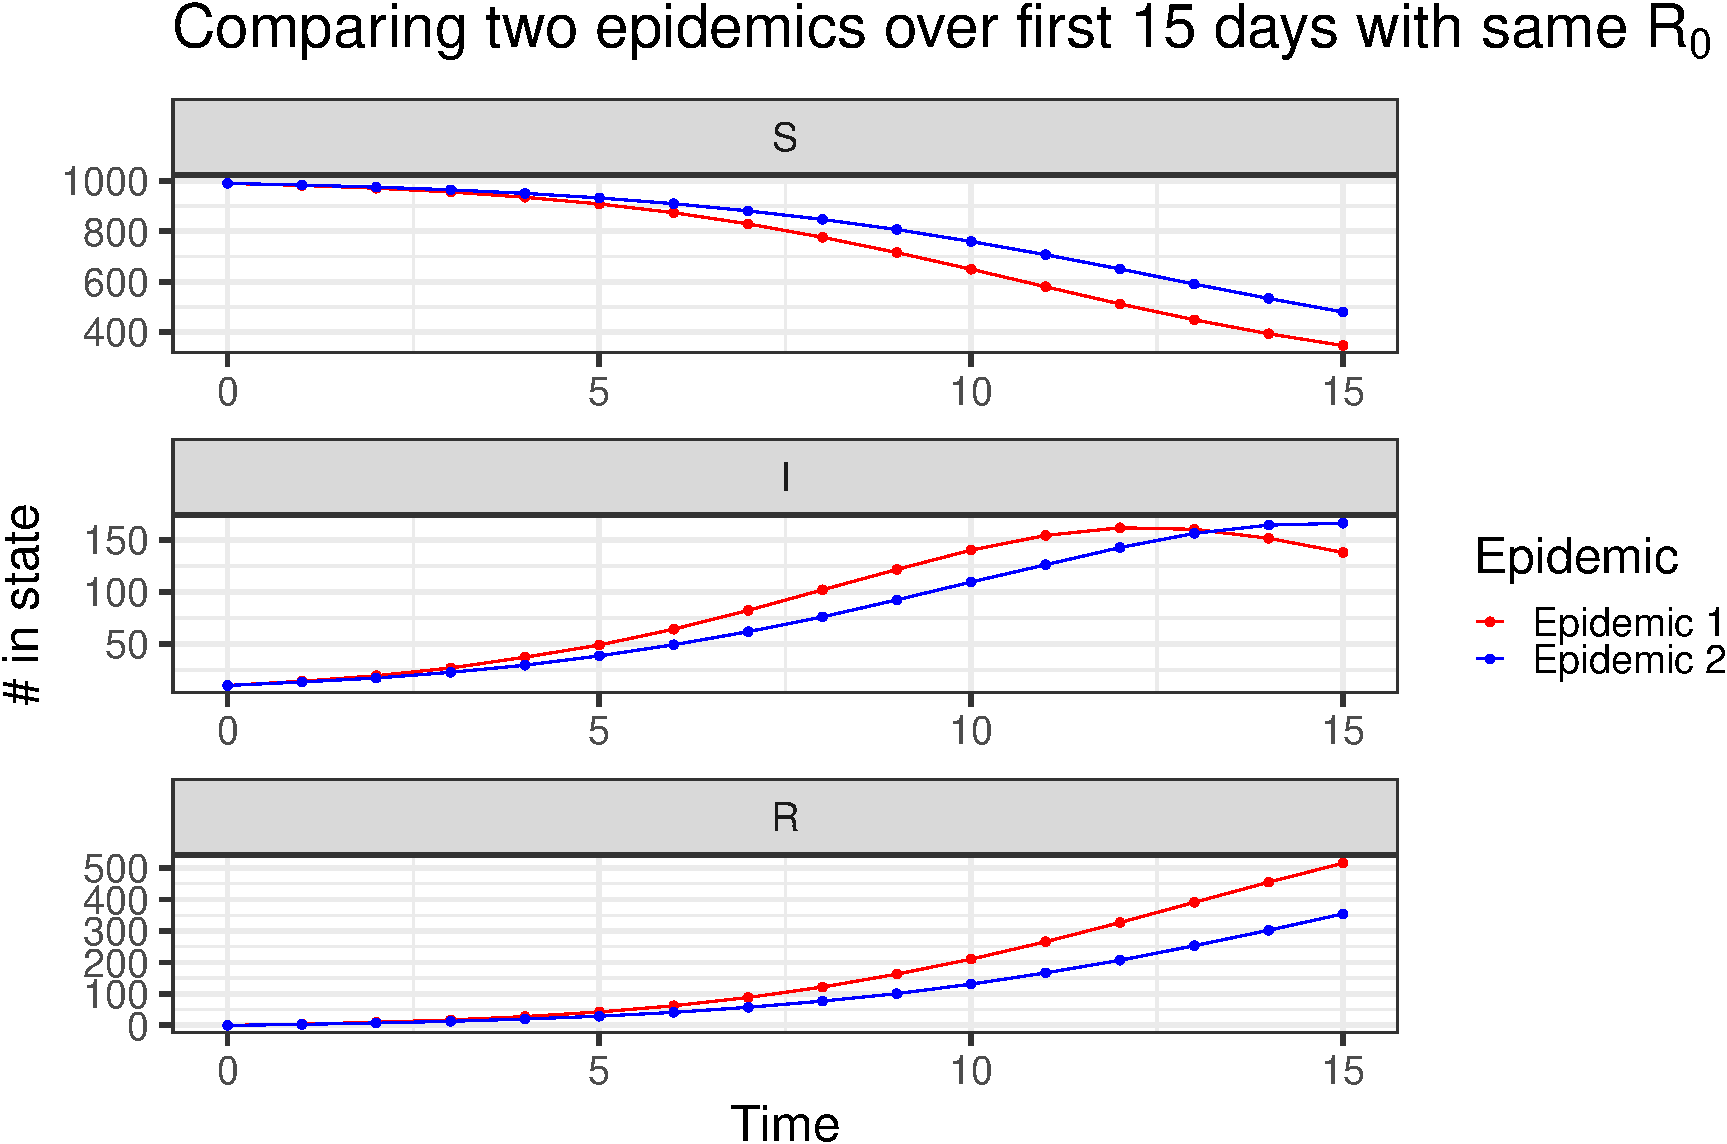
\includegraphics{Figs/unnamed-chunk-2-1} 

}

\caption{\label{fig:different-scales-standard}Example of two epidemics with different $\beta$ and $\gamma$ paremeters but the same initial reproduction number $R_0$ = 2.  Both epidemics are generated from models with $N= 1000$ individuals with $S(0) = 990$ and $I(0) = 10$.}\label{fig:unnamed-chunk-2}
\end{figure}
\end{CodeChunk}

\textcolor{blue}{\pkg{EpiCompare} provides a time-invariant tool to visualize these epidemics in a more intuitive manner, at least in regards to comparing values of $R_0$.}
\sout{A time-invariant approach to visualizing epidemics, in comparison, allows us to directly compare $R_0$ from a single plot.}
\textcolor{violet}{For every time \sout{point} $t$ we have a \textcolor{orange}{point} $(S(t),I(t), R(t))$\sout{, so we can treat epidemics as a trajectory in this three-dimensional space, as we visual in the left subplot of Figure \ref{fig:different-sacles-tern}.} \textcolor{orange}{so we can visualize the trajectory of the epidemic in three-dimensional space (see Fig. \ref{fig:different-scales-tern} (left)).} For state space models like in our example, given the constraint that $S(t) + I(t)+R(t)$ is always equal to $N$ (the total population size), we can visual these point in a a two-dimesional \textit{ternary} plot, as seen in Figure \ref{fig:different-scales-tern} (right). \sout{In Fig. \ref{fig:different-scales-tern}
we plot the filamental trajectories of the two epidemics in a time-invariant view. We will explain how and why this works shortly. The important takeaway is that in this time-invariant view, i}I}t
is apparent that these epidemics are on ``the same path.'' In this case,
this indicates that two epidemics have the same value of \(R_0\).

\begin{CodeChunk}
\begin{figure}[H]

{\centering 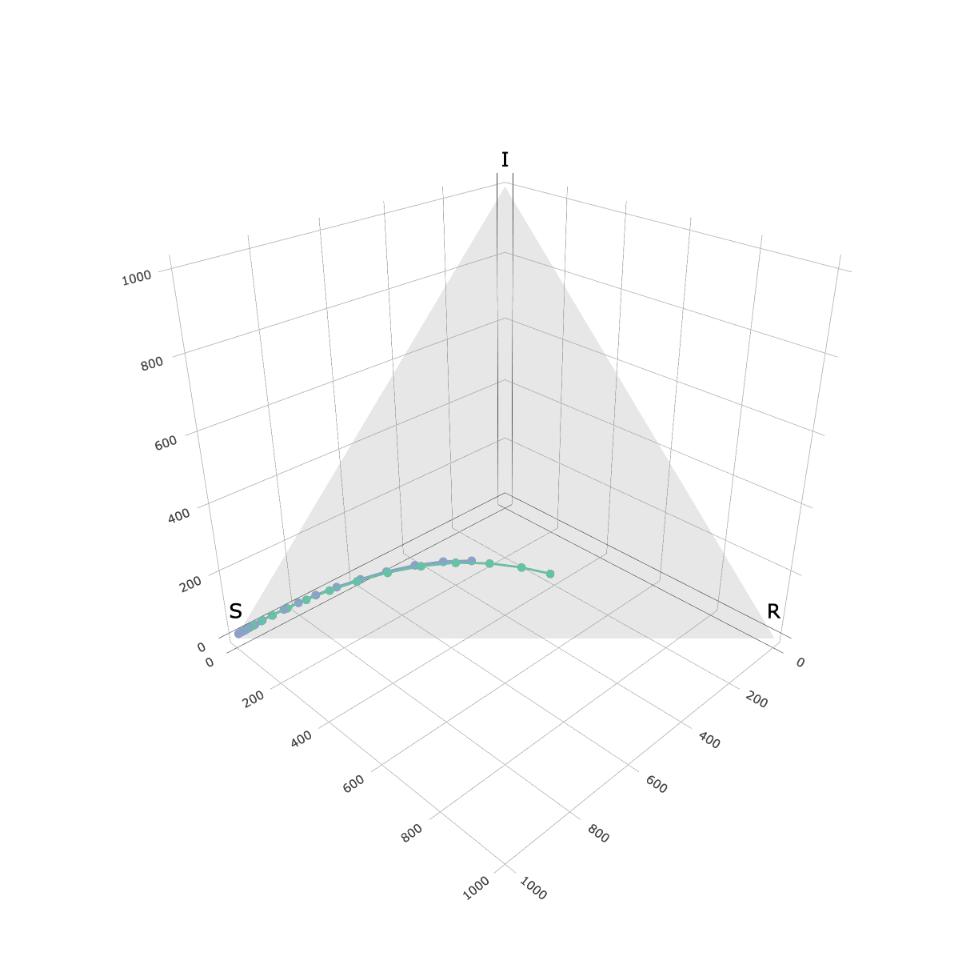
\includegraphics[width=0.49\linewidth]{images/vis3d} 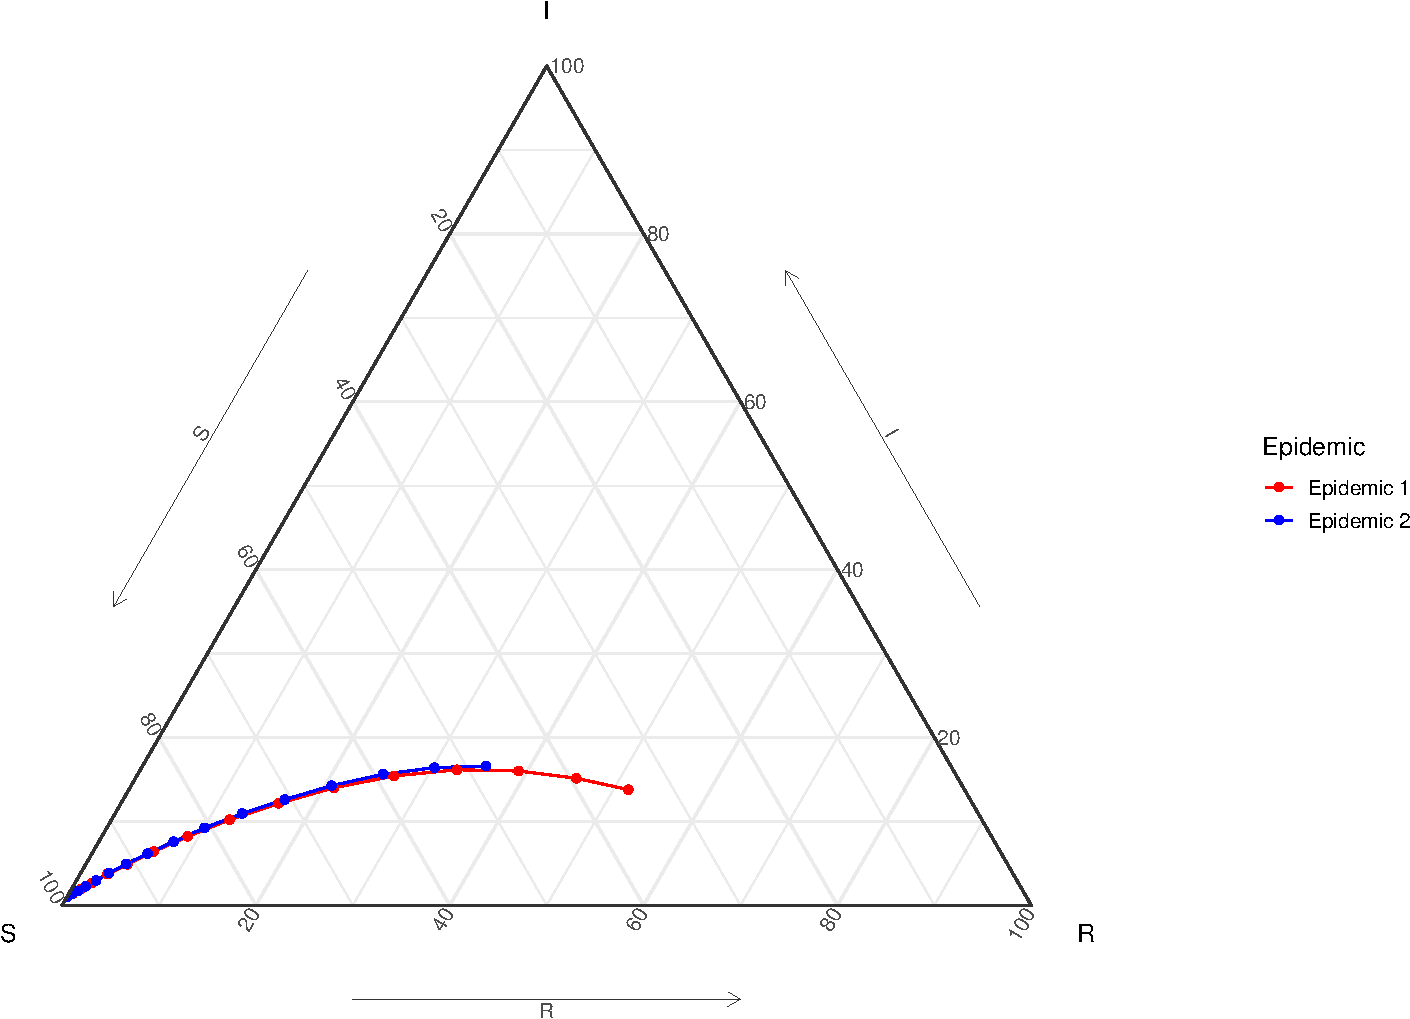
\includegraphics[width=0.49\linewidth]{Figs/unnamed-chunk-3-2} 

}

\caption{\label{fig:different-scales-tern}Left: trajectory of epidemic in three-dimensional space, plotting $(S(t), I(t), R(t))$.  Right: the gray-shaded region and epidemic trajectory shown from (left) now shown in two-dimensional space.  This is more commonly known as a ternary plot.}\label{fig:unnamed-chunk-3}
\end{figure}
\end{CodeChunk}

\textcolor{violet}{Underlying our time-invariant visualization that allowed for the comparison of $R_0$ in Fig. \ref{fig:different-scales-tern} is the treatment of the epidemic as a single filamental trajectory in the state space. \sout{The reason why we can visually compare $R_0$ in Fig. \ref{fig:different-scales-tern} is because of the time-invariant nature of the filamental trajectory associated with an epidemic.}}
A filamental trajectory can be mathematically viewed as a set of points
in space that have an ordering, and that all points on the line between
these ordered points are also contained in the geometric object. For a
SIR epidemic, we can represent the associated filamental trajectory
\(\psi\) as

\[
\psi = \left \{(S(t), I(t), R(t)): S, I, R \ge 0, S + I + R = N \right \}_{t\in[0,T]},
\] where a mapping \(\xi : s \to \mathbb{R}\) that is strictly
monotonically increasing would not change the definition of \(\psi\),
i.e.~\(\psi_\xi \equiv \psi\) where :

\[
\psi_\xi = \left \{(S(\xi(s)), I(\xi(s)), R(\xi(s))): S, I, R \ge 0, S + I + R = N \right \}_{s\in[0,T]}.
\] \textcolor{violet}{[Ben says: removed this paragraph now]} Since the
number \textcolor{orange}{of individuals} in each state is non-negative
and the sum over the three states for a given time point
\sout{sums to}\textcolor{orange}{is} \(N\), then
\textcolor{violet}{all points in} \(\psi\) will lay in a
\textbackslash ben\{two-dimensional triangular plane in
three-dimensional space.
\sout{We can then which can be visualize the \textcolor{orange}{full filamental trajectory} in a two-dimensional ternary plot}
As a result, we can visualize
\textcolor{orange}{the full filamental trajectory} of an epidemic in a
single
\textcolor{violet}{ternary plot \sout{2d plot and ultimately $R_0$}}.
\textcolor{orange}{[Shannon says: Show pic here?]}{]}\footnote{Which?  \textcolor{orange}{3d space one? But I'm leaning against it now.   3d never looks good in a paper.}}

\sout{\textcolor{violet}{[This section could be a bit less wordy. But generally good.]} We visualize the two epidemics in a global, ternary view in Figure \ref{fig:different-scales-tern}.  Without getting into too much detail of the intricacies of this plot, we immediately see the points of the two filaments $\psi$ seem to form the same trajectory.  Now, it is much clearer that \textcolor{violet}{\sout{Model} epidemic} 2 is following the same trajectory as \textcolor{violet}{\sout{Model} epidemic} 1 but is not as far along in the infection process. }

\sout{\textcolor{violet}{As suggested a few paragraphs back, t}}The
filamental trajectories in Fig. \ref{fig:different-scales-tern}
\sout{seem to overlap}, and we may suspect that something is
fundamentally linking these two different epidemics together.
Mathematically, we can show this fundamental link \sout{turns} is
\(R_0\). Let our two epidemics be presented as
\(\{(S_1(t), I_1(t), R_1(t))\}_{t\geq0}\),
\(\{(S_2(s), I_2(s), R_2(s))\}_{s \geq 0}\) respectively. As with the
example, assume both models have the same initial values
\((S(0), I(0), R(0))\), and let
\(R_0 =\frac{\beta_1}{\gamma_1} = \frac{\beta_2}{\gamma_2}\) where
\(\beta_i\) and \(\gamma_i\) are the average infection rate and recovery
rate, respectively, for SIR model \(i=1, 2\). And define \(a>0\) to be
the relative scalar such that \(\beta_2 = a \beta_1\) if and only if
\(\gamma_2 = a \gamma_1\).

\begin{theorem}\label{thm:sir-scale}
Let there be two SIR models as described above.  Then for all $t > 0$ there exists an $s>0$ such that $(S_1(t), I_1(t), R_1(t)) = (S_2(s), I_2(s), R_2(s))$.  Moreover, $s = \frac{1}{a}t$.
\end{theorem}

The proof of Theorem \ref{thm:sir-scale} relies on a fairly recent
result from \cite{Harko2014} and is shown in detail in Proof
\ref{proof:thm}. The consequence of Theorem \ref{thm:sir-scale} is that
for two SIR models that have the same initial percent of individuals in
each state and \(R_0\) then for every point on the epidemic path of the
first SIR model \textcolor{violet}{\sout{is also} can be mapped to} a
point on the epidemic path of the second SIR model.
\textcolor{orange}{In other words, the two epidemics form the same filamental trajectory. For SIR models with similar initial state percentages, time-invariant analysis allows practitioners to compare values of $R_0$ at a glance.}

\subsection[Beyond R0 and SIR]{Time-invariant analysis beyond \(R_0\)
and \sout{Kermack’s and McKendrick} SIR
Models\footnote{Probably will need to change this title...}}\label{sec:beyond-r0-sir}

Through the \(R_0\) example, we see that treating epidemics like
filamental trajectories embedded in a lower dimensional space allows us
to \sout{better}\textcolor{orange}{more fully} compare the overall
structure of the epidemic and see how the population is directly
impacted. Time-invariant tools \sout{that} can be useful even when the
underlying generative model for the epidemic is unknown or have more
than three epidemic states.

\textcolor{violet}{New paragraph} Viewing epidemics as filamental
trajectories provides \sout{a lot }new ways to compare and examine
epidemics in a time-invariant manner. \textbackslash ben\{For
\textcolor{orange}{completed?}epidemics that have ended, one way to
examine their filamental trajectories is to
\sout{redefine}\textcolor{orange}{represent} the
\textcolor{orange}{filamental} trajectory as a
\textcolor{orange}{finite sequence of equally spaced points.}
\sout{finite sequence of points on the filamental trajectory that are equally spaced (i.e. equa-distance between pairs of ordered points).}
\sout{For epidemics that have "played" themselves out, one way to represent their filamental trajectories to avoid \textcolor{orange}{confusion stemming from}\sout{impacts of} temporal structure is to define them as a sequence of points their trajectory with equi-distance between each point \textcolor{orange}{[Shannon says: are we missing a few words in this definition?]}}.
This representation induces a natural distance between this type of
representation between epidemics, specifically: \[
d_\text{equi-distance}(\psi_1, \psi_2)  = \int_{s \in [0,1]} (\psi_1'(s) - \psi_2'(s))^2 ds
\] where \(\psi_i'(s)\) the point along \(\psi_1\) that is \(s\)
fraction of \(|\psi_1|\) distance away from the start of
\(\psi_i\).\footnote{\textcolor{orange}{I think you're trying to say something about a distance based on the equally space points.  Some clarifying questions:  is $\psi^\prime$ the derivative?  Does proportion make more sense than fraction? or simply $\frac{|\psi|}{s}$? It's only naturally time-invariant if we have a well defined ending point, right?}}
This distance is naturally time-invariant, and can be plugged into
multiple distance-based assessment tools to examine the overall
``extremeness'\,' of points, including pseudo-density estimators and
depth/local depth functions
\citep[for examples see][]{Ciollaro2016, Geenens2017}. These extremeness
estimators can be \sout{very} useful when comparing
\sout{between a setof simulation} \textcolor{orange}{a set of simulated}
epidemics and the true
epidemic\textcolor{orange}{. Moreover these extremness estimators,}
\sout{and does} \textcolor{orange}{} not constrain the number of states
of the
model\sout{, though we recommend projecting the points into the unit simplex}\footnote{\textcolor{violet}{I'm not sure we've talked about this before... \textcolor{orange}{I don't think we have but am wondering if we're getting in the weeds}}}\sout{(by making all values the proportion of the population in the given state)}.

\textcolor{violet}{New paragraph:}
\textcolor{violet}{\sout{If the set of epidemics that one is examining have only gone through a single cycle of the outbreak} If \sout{one} \textcolor{orange}{a practicioner} is interested in understanding \textcolor{orange}{an} epidemic\sout{s} through a single \sout{cycle}\textcolor{orange}{realization} of \sout{their}\textcolor{orange}{its} outbreak}
(before the population of individuals have become susceptible again),
then additional time-invariant tools, including prediction regions can
be leveraged \textcolor{orange}{awk sentence}\footnote{\{\textcolor{orange}{What are we predicting if the epidemic is done? Update 4/6: I'm satisfied.}\}}.
In these settings, \textcolor{orange}{\pkg{EpiCompare} goes}
\sout{we go }a step further and treats epidemics more like geometric
filaments
\textcolor{orange}{(i.e. filamental trajectories without an ordering of points)}
than filamental trajectories. In \pkg{EpiCompare}, we create prediction
regions that contain a the top (\(1-\alpha\)) proportion of simulated
curves by defining geometric regions defined by the union of small
\textcolor{orange}{geometric?} filaments around the subset of
simulations (\sout{subset} \textcolor{orange}{grouped} by measures like
the above pseudo-density estimates or depth estimates). These regions
\sout{look at}\textcolor{orange}{show} where in the state-space we
expect the epidemic to traverse\sout{, and }.
\textcolor{orange}{Additionally, }we can compare prediction regions
defined by different models using
\textcolor{violet}{many set difference distances \sout{the Haussdorf \textcolor{orange}{why Haussdorf specifically?} distance}}
as well as examining how well the truth epidemic matches the simulations
by examining if the epidemic's trajectory lies within the prediction
region. All these \textcolor{orange}{mentioned?} geometric structures
and distance notations apply to epidemics with any number of states, and
at the end of Section \ref{sec:overview} we \sout{also} highlight how
these prediction regions can aid in visual comparisons for epidemics
with 3 states (like the SIR models).

\section[Package overview]{Overview of
\pkg{EpiCompare}}\label{sec:overview}

\afterpage{\clearpage}
\begin{sidewaysfigure}[!ht]
    \centering
    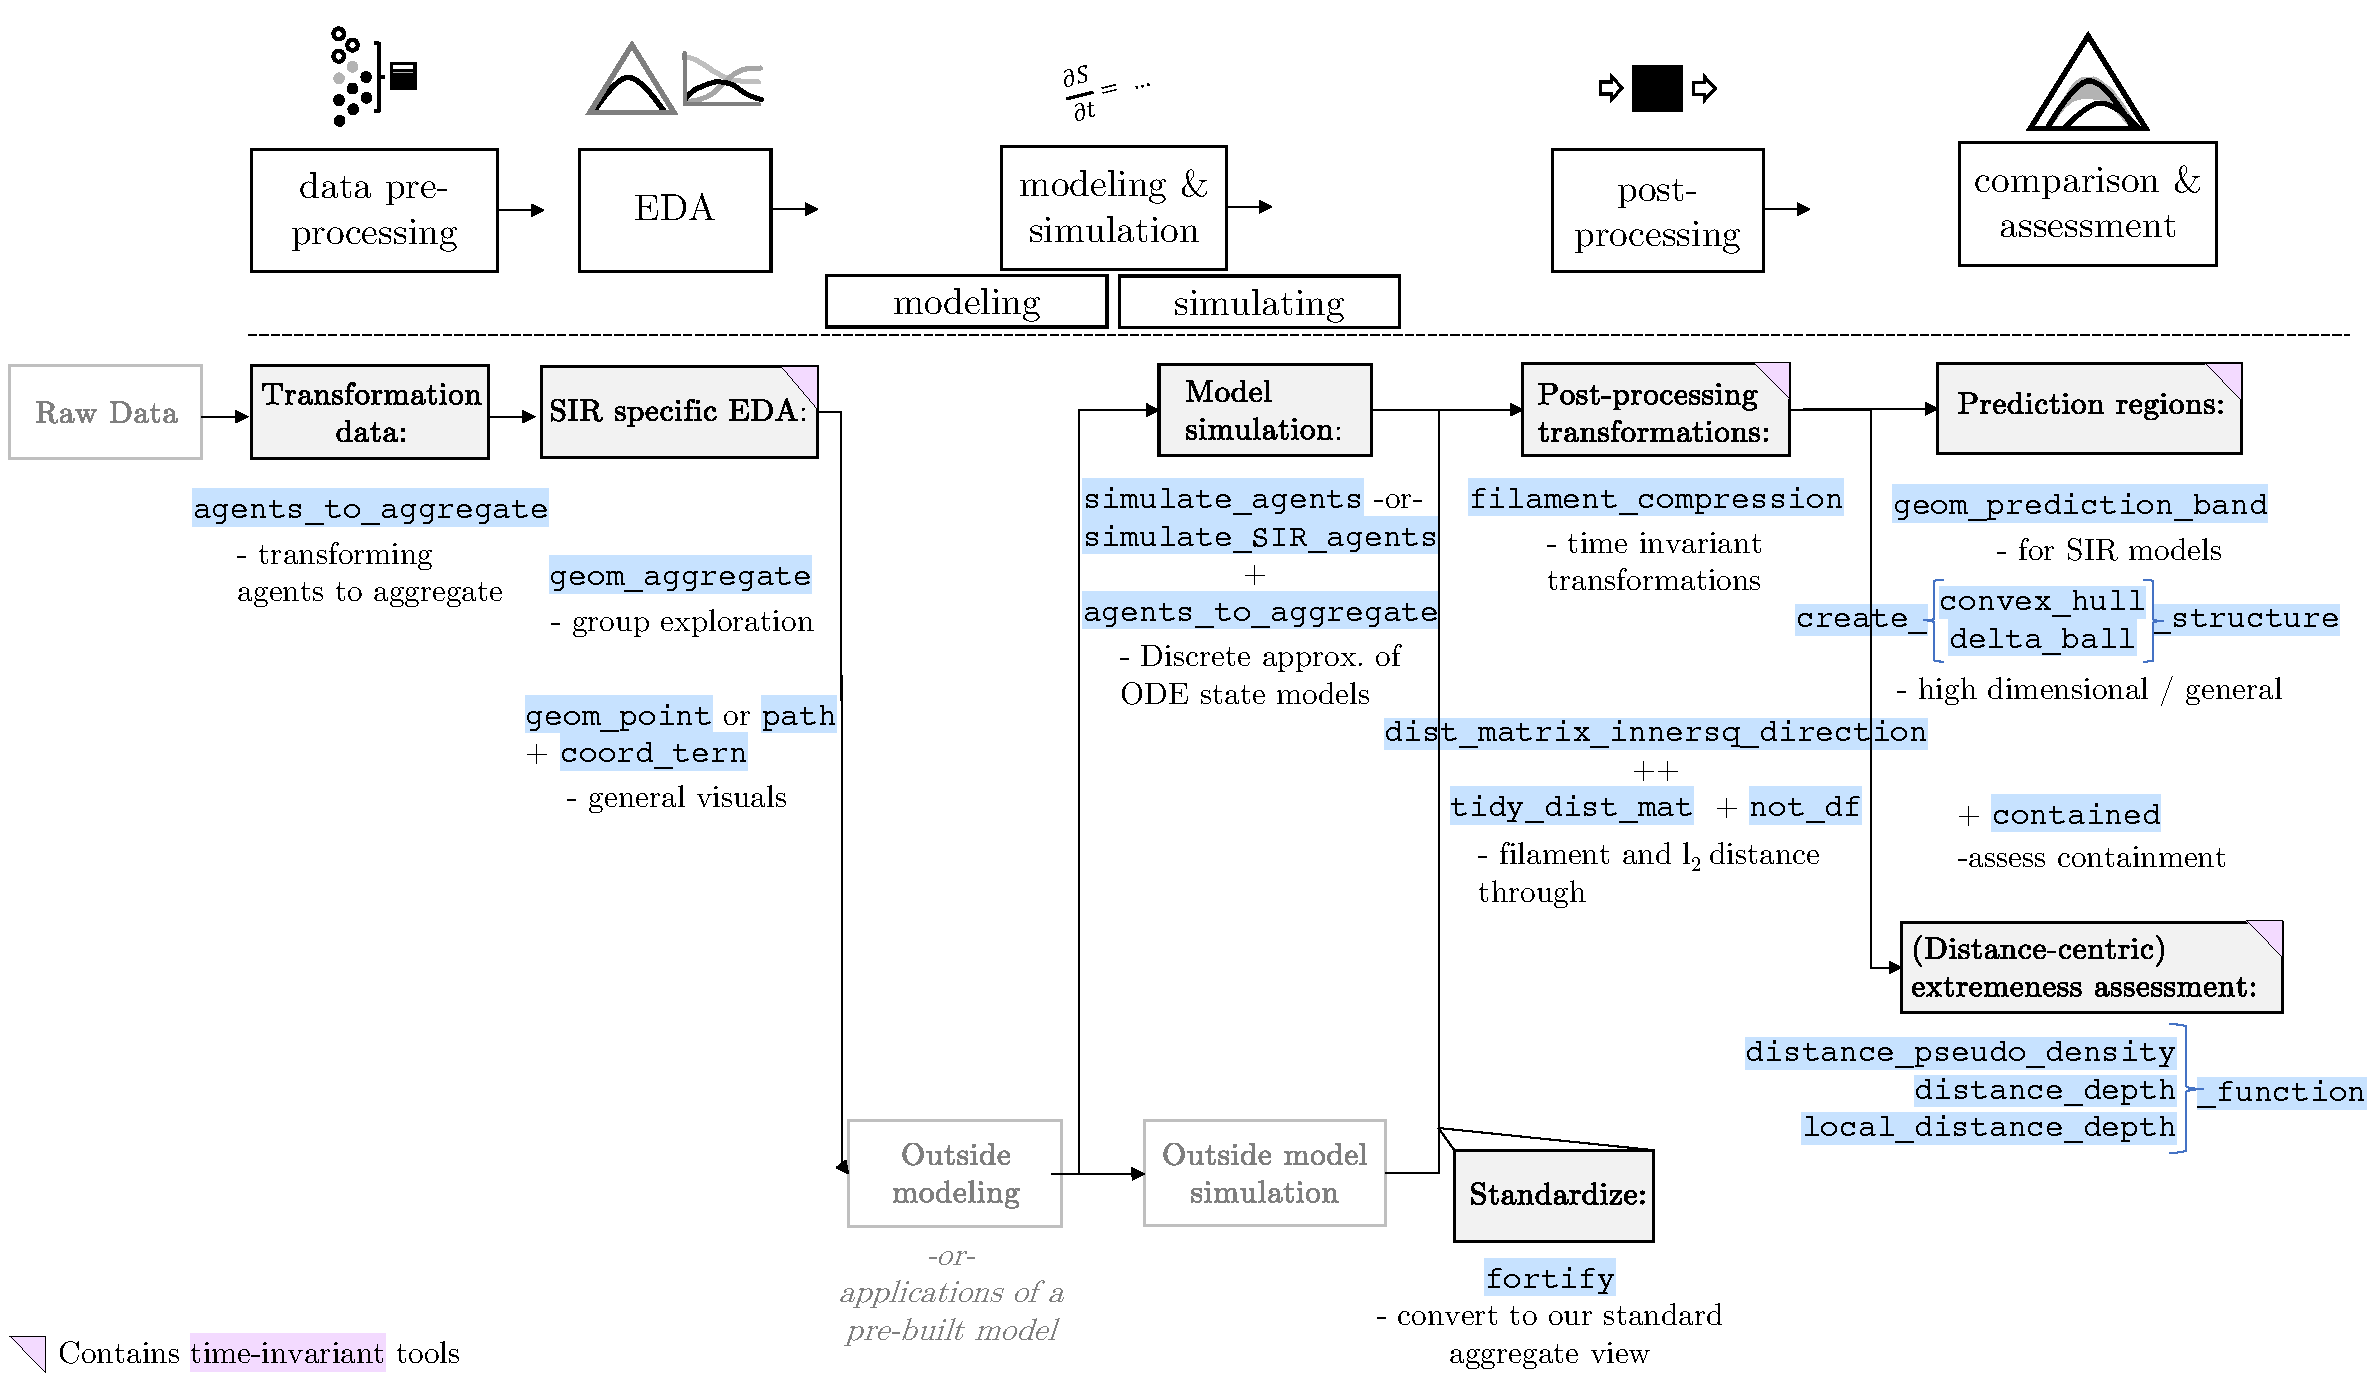
\includegraphics[width = 1\textwidth]{images/pipeline2_1.pdf}
    \caption{How \pkg{EpiCompare} supplements and aids in the epidemiological data analysis pipeline.}
    \label{fig:pipeline2}
\end{sidewaysfigure}

In this section, we present the tools implemented in \pkg{EpiCompare}
and explain how they aid in the data analysis pipeline. In Figure
\ref{fig:pipeline2}, we show how our package's functions fit into the
data analysis pipeline introduced in Figure \ref{fig:pipeline}. All
front-facing functions in \pkg{EpiCompare} are aimed to be as
user-friendly as possible. We also focus on providing the user
``tidyverse'' style functions, that encourage piping objects from one
function to the next and follow clear ``verb'' naming schemes
\citep{Wickham2019}. Although users can incorporate \pkg{EpiCompare}
into any step in the data analysis pipeline, there are two primary
points of entry. The first point of entry is the very beginning with
pre-processing and visualizing raw data, and the second point of entry
is after modeling and simulation. Figure \ref{fig:pipeline2} captures
these different paths, and we highlight how to leverage \pkg{EpiCompare}
functionalities in the subsections below.

\textbf{Data pre-processing}

The first step of most data analysis is ``cleaning'' the raw data so it
can be explored. Before data can be explored, they must be collected.
Sometimes individual records are collected, with times of different
states of the epidemic (infection, recovery, etc.) as well as individual
information like network structure, location, and sub-population
information. Other data collections focus on aggregate counts of
individuals in each epidemic state. In fact, many times only the number
of new infections at each time step (e.g.~weekly case counts) is
observed. In this setting, compartment totals (amounts of individuals in
each state) are then imputed from those case counts and using other
information about the disease and the population of interest. In
\pkg{EpiCompare}, we focus on understanding the overall impact of an
outbreak at the aggregate/population level, which allows for streamlined
examination of overall trends of an epidemic.

To help the practitioner examine epidemics from an aggregate/population
lens, we provide a function called \texttt{agents\_to\_aggregate()}.
This function transforms data about individual/agents' initial entry
into each state (e.g.~start of infection, start of recovery, etc.) to an
aggregate view of how many individuals were in a state at a given time.
Researchers, including \citet{rvachev1985,anderson1992,worby2015}, often
are interesting in more granular trends that can be detected by
aggregation, conditional on subpopulations (e.g.~subpopulations defined
by age or sex). By combining the function
\pkg{dplyr}::\texttt{group\_by()} and \texttt{agents\_to\_aggregate()},
\pkg{EpiCompare} provides group level aggregation.

Besides aiding subpopulation analysis, \texttt{agents\_to\_aggregate()}
can accommodate a wide range of information about each individual. In
fact, this function can account for infinitely many states. This
functionality allows the practitioner to aggregate information relative
to common states (e.g.~``Susceptible'', ``Infectious'', and
``Recovered'') as well as more complex states (e.g.~``Exposed'',
``iMmune'', ``Hospitalized''). Additionally,
\texttt{agents\_to\_aggregate()} permits indicators for death/exit and
birth/entry dates. Overall, this function is a powerful tool for
pre-processing data.

\textbf{Exploratory data analysis (EDA)}

In the early stages of a project, familiarizing oneself with the data
usually means figuring out useful combinations of visualizations and
numerical summaries of the data both at population and subpopulation
level. An expert coder can start with \texttt{agents\_to\_aggregate()}
to successfully accomplish exploratory data analysis (EDA) in many ways.
\pkg{EpiCompare} also includes tools that allow a novice coder to
rapidly explore data, provided there are three unique epidemiological
states (like in the SIR model). Building on \pkg{ggplot2} and
\pkg{ggtern} packages, \pkg{EpiCompare}'s \texttt{geom\_aggregate()}
provides a way to explore how different subpopulations experience of an
epidemic \citep{Wickham2016, Hamilton2018}. The function
\texttt{geom\_aggregate()} provides a visualization tool to holistically
examine aggregate level information across different subpopulations by
visualizing each subpopulation's epidemic trajectory in the
three-dimensional state space. Visualization tools for three-state
models were developed because SIR models are some of the most common and
basic epidemic state-based models and our three-dimensional simplex
representation of these epidemics emphasizes a time-invariant
representation of the data (for a refresher see Section
\ref{sec:time-invariant}).

\textbf{Model fitting and simulations}

After getting a sense of what a past or current epidemic looks like with
EDA, the next step in the data analysis pipeline is often model fitting
and/or simulation. While \pkg{EpiCompare} does not focus on fitting
models to data, we do provide some flexible functions for simulation of
basic discrete-time epidemic-state models. These functions simulate
individual-level information based on practitioner estimated transition
rates between states and can be combined with
\texttt{agents\_to\_aggregate()} to view these simulations through an
aggregate lens. The function \texttt{simulate\_SIR\_agents()} simulates
a basic SIR epidemic with user inputs for the number of simulations, the
initial number in each state, the infection and recovery parameters
\((\beta, \gamma\)), and the total number of discrete time steps. Beyond
SIR models, the function \texttt{simulate\_agents()} takes as input a
user-specified state-transition matrix and other epidemic parameters to
allow the user to create simulations for an outbreak with \textit{any}
number of states and any number of transitions among them. This
flexibility in states can be used to also reflect group-based dynamics.
Both of these functions allow users to explore the space of models in an
intuitive way without getting bogged down by too much mathematical
detail. For consistency, we have made output from
\texttt{simulate\_agents()} and \texttt{simulate\_SIR\_agents()}
compatible with \texttt{agents\_to\_aggregate()} so aggregate
information may easily be accessed.

\textbf{Post-processing}

If practitioners wish to compare models-to-observations or even
models-to-models, they need to post-process their models and simulations
to disseminate the results in an easily digestible format. In
\pkg{EpiCompare}, we provide (1) functions to standardize simulation and
model output from external packages and (2) a function to transform
standardized simulation and model output into a format amenable to
time-invariant analysis.

Modeling and simulation output can be very complex objects, and as a
result, a number of epidemic modeling \proglang{R} packages return a
special class. The special classes often contain a plethora of
information about residuals, model diagnostics, input parameters, and
more. While incredibly useful, these special classes can be difficult
for novice coders to handle. To this end, \pkg{EpiCompare} provides a
series of fortify-style methods, called \code{fortify_aggregate()} which
transform output from infectious disease modeling and simulation
packages like \pkg{pomp} and \pkg{EpiModel} into tidy-styled data frames
which contain information about the total number of individuals in each
state at a given time, for a given simulation. These fortify functions
have output that is consistent with that of
\code{agents_to_aggregate()}. These standardized outputs can then be
piped to summaries, tables, and plots.

Because epidemic data is stored in a temporal way, we provide the
function, \code{filament_compression()}, to transform temporally defined
epidemics to their filamental representations. These filaments can then
be fairly compared to one another or passed to further time-invariant
analysis tools described below.

\textbf{Comparisons and assessment} \textcolor{orange}{[[ NEW TEXT}

\textcolor{violet}{\sout{Finally,} Often}\footnote{\textcolor{violet}{[Ben says: I feel like starting with "finally" causes a weird pause - but maybe that's just me.]}}
the data analysis pipeline \textcolor{violet}{\sout{often}} ends with
plots, tables, and summary statistics that are used to
\sout{\textcolor{violet}{compare} \textcolor{orange}{and assess}}
\textcolor{violet}{\sout{different models, and simulations to one another} assess model preformance and compare across models or simulations.}
In \pkg{EpiCompare} we provide a set of comparison and assessment tools
for model and simulation results that extend beyond the standard
performance metrics (e.g.~mean squared error or AIC) and into the lens
of time-invariant analysis. We have found \textcolor{violet}{that} these
tools \textcolor{violet}{\sout{to be} are} specifically applicable for
situations where only one season or cycle of an epidemic has occurred,
\textcolor{violet}{or is the object of interest}.

\footnote{\textcolor{violet}{[Ben says: This changed introduction was done to highlight that we can use prediction regions for mutiple types of comparisons.]}}\textcolor{violet}{The first set of of tools surround the creation of prediction regions. We can create a prediction regions from model simulations to examine if our model simulations capture the true epidemic trajectory. We do so in a time-invariant way and utilizing filamental representations of the model simulations and the true epidemic.}
{[}For three-state epidemic models, we provide the
\texttt{ggplot}/\texttt{ggtern} extension
\texttt{geom\_prediction\_band()} which creates a prediction region
around the top \(1-\alpha\) proportion of the simulations. In this
visual setting, comparing this prediction \textcolor{violet}{region} to
the true epidemic trajectory
\textcolor{violet}{\sout{or comparing the prediction regions defined by two different models' simulations}}\footnote{\textcolor{violet}{[Ben says: this part will be highlighted in later sentences.]}}
can be done by eye. In \pkg{EpiCompare}, we also provide these
prediction regions for epidemic models with with more than three states.
The functions \texttt{create\_convex\_hull\_structure()} and
\texttt{create\_delta\_ball\_structure()} create different geometric
representations of prediction regions for any dimensional state-based
model. For both of these geometric structures, we provide functions to
check if a path is contained (\texttt{contained()}){]}.
\textcolor{violet}{We can also use these prediction regions to visually or mathematically compare how similar two sets of simulations are. In \pkg{EpiCompare} we provide the}
\texttt{hausdorff\_dist()}
\textcolor{violet}{function to calculate the Hausdorff distance between multiple prediction regions, when visual comparison is not possible.}

{[}We also provide functions to calculate the ``extremeness'' of a true
epidemic trajectory compared to simulated epidemics via the
equi-distance filamental trajectory representation as mentioned in
Section \ref{sec:beyond-r0-sir}.{]}
\textcolor{violet}{We provide implementations of a few distance-based score functions that capture how "reasonable" an epidemic is relative to other epidemics, and these scores can be turned into an extremeness measure with}
\texttt{mean(sim\_scores\ \textgreater{}\ truth\_score)}.
{[}Specifically, functions like
\texttt{distance\_pseudo\_density\_function()} can calculate a
pseudo-density estimate of the true epidemic relative to simulated ones.
Functions \texttt{distance\_depth\_function()} and
\texttt{local\_distance\_depth\_function()} provide depth scores that
suggest how geometrically central an epidemic is to simulations.{]}

{]}{]}

{[}{[}\textcolor{red}{ OLD TEXT}

One tool we provide to assess models is through the creation of
geometric prediction regions, which are useful when we treat epidemics
like filaments. If there is a set of simulated epidemics from a model,
we can create a geometric prediction region for the expected trajectory
of the epidemic in the state space. For three-state epidemic models, we
provide the \texttt{ggplot}/\texttt{ggtern} extension
\texttt{geom\_prediction\_band()} which creates a prediction region
around the top \(1-\alpha\) proportion of the simulations. In this
visual setting, comparing this prediction to the true epidemic
trajectory or comparing the prediction regions defined by two different
models' simulations can be done by eye. In \pkg{EpiCompare}, we also
provide these prediction regions for epidemic models with with more than
three states. The functions \texttt{create\_convex\_hull\_structure()}
and \texttt{create\_delta\_ball\_structure()} create different geometric
representations of prediction regions for any dimensional state-based
model. For both of these geometric structures, we provide functions to
check if a path is contained (\texttt{contained()}) and the ability to
assess the Hausdorff distance between prediction regions based on
simulations from different model (\texttt{hausdorff\_dist()}). The
vignettes for \texttt{EpiCompare} go into much more mathematical detail
about how these functions can be used in conjunction with time-invariant
analysis.

We also provide functions to calculate the ``extremeness'' of a true
epidemic trajectory compared to simulated epidemics via the
equi-distance filamental trajectory representation as mentioned in
Section \ref{sec:beyond-r0-sir}. Specifically, functions like
\texttt{distance\_pseudo\_density\_function()} can calculate a
pseudo-density estimate of the true epidemic relative to simulated ones.
Functions \texttt{distance\_depth\_function()} and
\texttt{local\_distance\_depth\_function()} provide depth scores that
suggest how geometrically central an epidemic is to simulations.

\textcolor{orange}{]]}

{[}{[}\textcolor{red}{Really OLD TEXT}

Finally, in \pkg{EpiCompare} we provide a set of comparison and
assessment tools for model and simulation results that extend beyond the
standard performance metrics (e.g.~mean squared error or AIC).
Corresponding\footnote{\textcolor{violet}{[Ben says: "corresponding to" doesn't seem to be the correct phrase here. If we wanted to use "corresponding" I might imagine saying "corresponding to the araguments for time-invariant analysis in Section 2.2, EpiCompare provides such tools." I'm open to keeping it if you think it's the perfect word choice.]}\textcolor{orange}{"To support the ideas presented in Sec."?}}
to Section \ref{sec:beyond-r0-sir}, \pkg{EpiCompare} provides a set of
time-invariant tools to compare and evaluate epidemic models and
simulations. We have found these tools to be specifically applicable for
situations where only one ``season'' or
``cycle''\footnote{\textcolor{violet}{[Ben says: I think we can remove the paratheses here.]} \textcolor{orange}{accepted}}
of the epidemic has occurred.

\footnote{\textcolor{violet}{[Ben says: multiple parts of this paragraph might benefit with capturing a bit more of the motivation in the rewrite of Section 2 for the tools we're presenting.]}\textcolor{orange}{motivate better}}One
tool we provide to assess models is through the creation of geometric
prediction regions, which are useful when we treat epidemics like
filaments. If there is a set of simulated epidemics from a model, we can
create a geometric prediction region for the expected trajectory of the
epidemic in the state space. For three-state epidemic models, we provide
the \texttt{ggplot}/\texttt{ggtern} extension
\texttt{geom\_prediction\_band()} which creates a prediction region
around the top \(1-\alpha\) proportion of the simulations. In this
visual setting, comparing this prediction to the true epidemic
trajectory or comparing the prediction regions defined by two different
models' simulations can be done
\textcolor{violet}{by eye.\sout{with the 'eye test.'}\textcolor{orange}{I'm not saying 'no' but I'd do it in an appendix and not the main text.  I don't think equations belong in Section 3.}}
In \pkg{EpiCompare} we also provide these prediction regions for
epidemic models with with more than three states. The functions
\texttt{create\_convex\_hull\_structure()} and
\texttt{create\_delta\_ball\_structure()} create different geometric
representations of prediction regions for any dimensional state-based
model. For both of these geometric structures, we provide functions to
check if a path is contained (\texttt{contained()}) and the ability to
assess the Hausdorff distance between prediction regions based on
simulations from different model (\texttt{hausdorff\_dist()}).

\footnote{\textcolor{violet}{[Ben says: random thought (not needed) - maybe we do provide some equations for these measures and also maybe mathematically express how we'd examine extremeness?]}}We
also provide functions to calculate the ``extremeness'' of a true
epidemic trajectory compared to simulated epidemics via the
equi-distance filamental trajectory representation as mentioned in
Section \ref{sec:beyond-r0-sir}. Specifically, functions like
\texttt{distance\_pseudo\_density\_function()} can calculate a
pseudo-density estimate of the true epidemic relative to simulated ones.
Functions \texttt{distance\_depth\_function()} and
\texttt{local\_distance\_depth\_function()} provide depth scores that
suggest how geometrically central an epidemic is to simulations. {]}{]}

\section[Tour]{A tour of \pkg{EpiCompare}}\label{sec:tour}

\textcolor{orange}{[[NEWER TEXT}

To conclude our paper, we demonstrate the capabilities of
\pkg{EpiCompare} with a complete data analysis of a measles outbreak in
1861-1862 Germany. Specifically, we demonstrate how tools in
\pkg{EpiCompare} can be used in each step of the data analysis pipeline
(see Fig. \ref{fig:pipeline}). Additionally, we highlight how
time-invariant analysis (see Section \ref{sec:time-invariant}) can be
used to enhance understanding of an outbreak.

Before demonstrating \pkg{EpiCompare}, we provide some context for the
measles outbreak presented here. The data was originally organized by
\cite{pfeilsticker1863}, later made visible by \cite{oesterle1992}, and
made available in an \proglang{R} by \cite{surveillance2017}. This data
set includes a rich collection of features including household location,
class level, and allged infector ID, and is an ideal testing ground for
methodology in infectious disease epidemiology
\cite{Neal2004,britton2011,groendyke2012,becker2016}. In this data set,
there are 188 children who became infected with the measles over the
course approximately 90 days.

\textcolor{orange}{]]}

\textcolor{orange}{[[LESS NEW TEXT}

Finally, in this section we show how tools from \pkg{EpiCompare} can be
used in each step of the data analysis pipeline shown in Fig.
\ref{fig:pipeline}. We analyze an outbreak of measles in the town of
Hagelloch, Germany from 1861-1862, a data set organized by
\cite{pfeilsticker1863}. The data was later made visible by
\cite{oesterle1992} and made available in an \proglang{R} by
\cite{surveillance2017}. This data set includes a rich collection of
features and is an ideal testing ground for methodology in infectious
disease epidemiology
\cite{Neal2004,britton2011,groendyke2012,becker2016}.\footnote{\textcolor{orange}{The old first paragraph from data and exploratory analysis paragraph was combined with the intro as a better lead-in to what's going on.}}

\textcolor{orange}{]]}

{[}{[}\textcolor{red}{OLD TEXT}

\footnote{\textcolor{violet}{[Ben says: Shannon, would you mind reading this whole section over again once we've finished edits for section 2 and 3? This initial paragraph seems to be stating section 3's story.]}}In
this section, we highlight many of the tools available in
\pkg{EpiCompare}. As previously discussed, these tools include data
cleaning; visualization; modeling and simulation; post-processing; and
comparison and model assessment, in accordance with the data analysis
pipeline (Fig. \ref{fig:pipeline}). We show a full data analysis from
beginning to end that can be accomplished in a streamlined and
standardized manner via \pkg{EpiCompare}. {]}{]}

\subsection{Pre-processing and EDA}

\begin{CodeChunk}
\begin{table}[!h]

\caption{\label{tab:hags-people}Subset of Hagelloch infection data.  Features include the person ID, household ID (HH ID), age, sex, class level (Pre-K/1st/2nd), date of first symptoms, date of the appearance of the measles rash, and the alleged infector ID of the individual.}
\centering
\begin{tabular}[t]{rrlrllllr}
\toprule
ID & HH ID & Name & Age & Sex & Class & Symp. Start & Rash Date & Infector ID\\
\midrule
1 & 61 & Mueller & 7 & female & 1st class & 1861-11-21 & 1861-11-25 & 45\\
2 & 61 & Mueller & 6 & female & 1st class & 1861-11-23 & 1861-11-27 & 45\\
3 & 61 & Mueller & 4 & female & preschool & 1861-11-28 & 1861-12-02 & 172\\
4 & 62 & Seibold & 13 & male & 2nd class & 1861-11-27 & 1861-11-28 & 180\\
5 & 63 & Motzer & 8 & female & 1st class & 1861-11-22 & 1861-11-27 & 45\\
45 & 51 & Goehring & 7 & male & 1st class & 1861-11-11 & 1861-11-13 & 184\\
\bottomrule
\end{tabular}
\end{table}

\end{CodeChunk}

The Hagelloch data include a rich set of features at the individual
level,
\textcolor{orange}{and the tools in \pkg{EpiCompare} help with pre-processsing and EDA}.
Recorded features include household members, school level, household
locations, date of first symptoms (prodromes), date of measles rash, and
even the alleged infector. A subset of the data is shown in Table
\ref{tab:hags-people}. \textcolor{orange}{For example,} with
\pkg{EpiCompare}, we can easily
\textcolor{orange}{pre-process the data to} obtain the empirical
cumulative incidence function with respect to the measles rash
appearance (variable \code{ERU}) with the following tidy-style function,
\code{agents_to_aggregate()}. The function \code{agents_to_aggregate()}
is a key component of \pkg{EpiCompare}, allowing the user to easily
switch from an individual-level (i.e.~an agent) \sout{view} lens of a
disease to an aggregate \sout{level} lens. For example, the below code
shows how we can convert the agent data to a cumulative incidence
\textcolor{orange}{plot} of the measles
rash\sout{, in order to see how the disease spread through the population over time.}
We can then compare the cumulative incidence of the rash to the
cumulative incidence of the prodromes, i.e.~the initial symptoms. We do
this with the below code, and a part of the cumulative incidence data
output is shown in Table \ref{tab:cif-rash}. The argument
\code{integer_time_expansion} indicates whether we should include all
time points in the recorded range of the data or only when there is a
change in the incidence.

\begin{CodeChunk}
\begin{CodeInput}
R> cif_rash  <- hagelloch_raw %>%
+   mutate(time_of_rash = as.numeric(ERU - min(PRO, na.rm = TRUE))) %>%
+   agents_to_aggregate(states = time_of_rash,
+                       integer_time_expansion = FALSE) %>%
+   mutate(type = "Rash")
\end{CodeInput}
\end{CodeChunk}

\begin{CodeChunk}
\begin{table}[!h]

\caption{\label{tab:cif-rash}Turning the individual-level information from the Hagelloch data to an aggregate view of the cumulative incidence of the measles rash in the population over time.}
\centering
\begin{tabular}[t]{rrr}
\toprule
Time & \# Susceptible & \# Total rash appearances\\
\midrule
0 & 188 & 0\\
4 & 187 & 1\\
7 & 186 & 2\\
9 & 185 & 3\\
12 & 183 & 5\\
\bottomrule
\end{tabular}
\end{table}

\end{CodeChunk}

One possible question of interest is the duration between initial onset
of prodromes and the appearance of the measles rash. Since
\code{agents_to_aggregate()} outputs a tidy-style data frame, it is a
simple task to plot the two sets of incidence curves on the same graph
(Fig. \ref{fig:cifs}).

\begin{CodeChunk}
\begin{CodeInput}
R> cif_prodromes <- hagelloch_raw %>%
+   mutate(time_of_PRO = as.numeric(PRO - min(PRO, na.rm = TRUE))) %>%
+   agents_to_aggregate(states = time_of_PRO,
+                       integer_time_expansion = FALSE) %>%
+   mutate(type = "Pro")
\end{CodeInput}
\end{CodeChunk}

\begin{CodeChunk}
\begin{CodeInput}
R> plot_df <- bind_rows(cif_rash, cif_prodromes)
R> 
R> ggplot(data = plot_df,
+        aes(x = t, y = X1, col = type)) + 
+   geom_step() + 
+   labs(title = "Cumulative incidence of measles appearance",
+        x = "Time (days relative to first prodrome appearance)",
+        y = "Cumulative incidence of event") + 
+   coord_cartesian(xlim = c(0, 55)) +
+   scale_color_manual(values = c("blue", "red"))
\end{CodeInput}
\begin{figure}[H]

{\centering 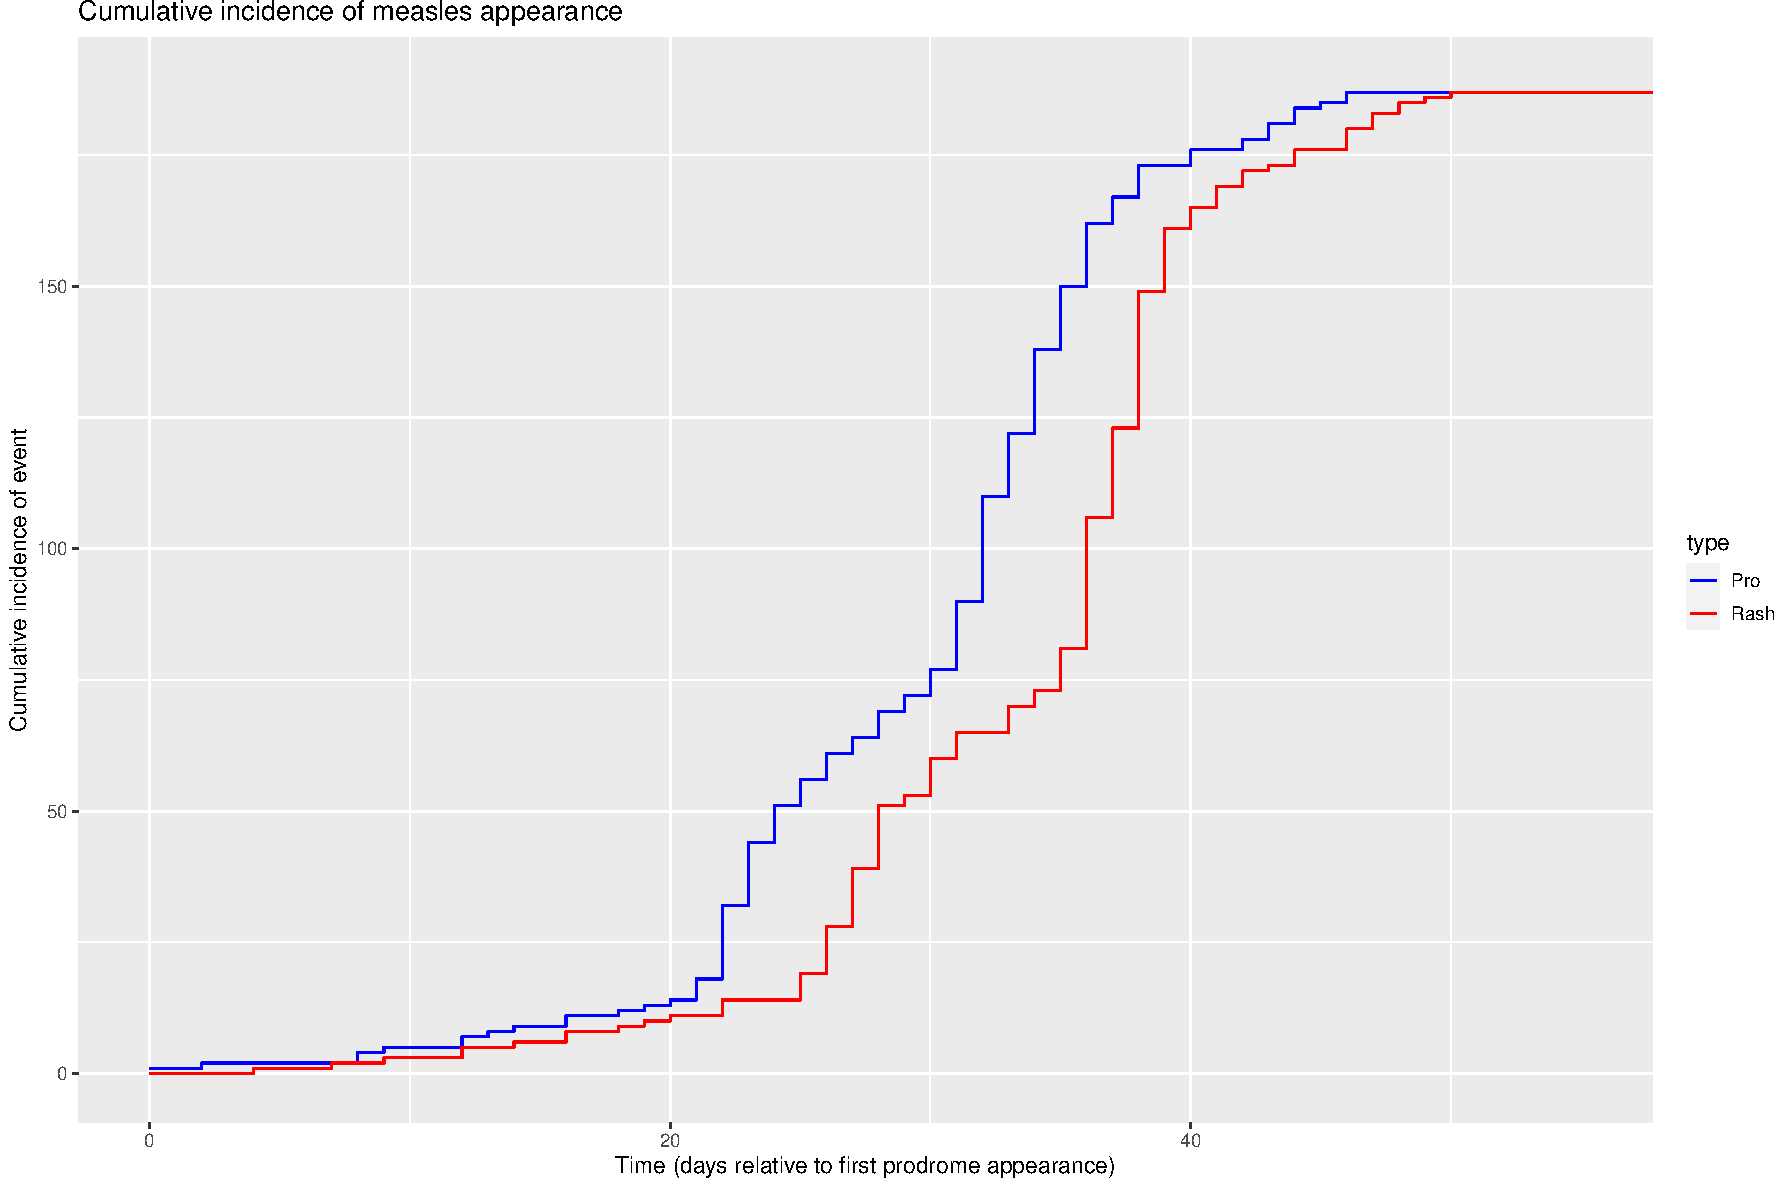
\includegraphics{Figs/unnamed-chunk-7-1} 

}

\caption{\label{fig:cifs}Empirical cumulative incidence functions of prodrome (symptom) onset and measles rash appearance.  We see that there is approximately a a constant lag between the two curves.}\label{fig:unnamed-chunk-7}
\end{figure}
\end{CodeChunk}

The real power of \code{agents_to_aggregate()} lies in its ability to
aggregate over any number of pre-specified states. For example, the
Hagelloch data sets contains two columns, \code{tI} and \code{tR}, the
time of infection and recovery, respectively of each individual. We can
then plot the SIR values through a time-invariant lens using
\pkg{ggplot2} and \pkg{ggtern} functions (as shown in Fig.
\ref{fig:hag-tern-raw}) or with our custom \code{geom},
\code{geom_aggregate}, which takes the raw agent data as input.

\begin{CodeChunk}
\begin{CodeInput}
R> hagelloch_sir <- hagelloch_raw %>%
+   agents_to_aggregate(states = c(tI, tR),
+                       min_max_time = c(0, 55)) %>%
+   rename(time = t, S = X0, I = X1, R = X2)
R> 
R> 
R> ggplot(hagelloch_sir, aes(x = S, y = I, z = R))+
+   coord_tern() +
+   geom_path() +
+   labs(x = "S", y = "I", z = "R",
+        title = "Time invariant view of Hagelloch measles outbreak") + 
+   theme_sir(base_size = 24)
\end{CodeInput}
\begin{figure}[H]

{\centering 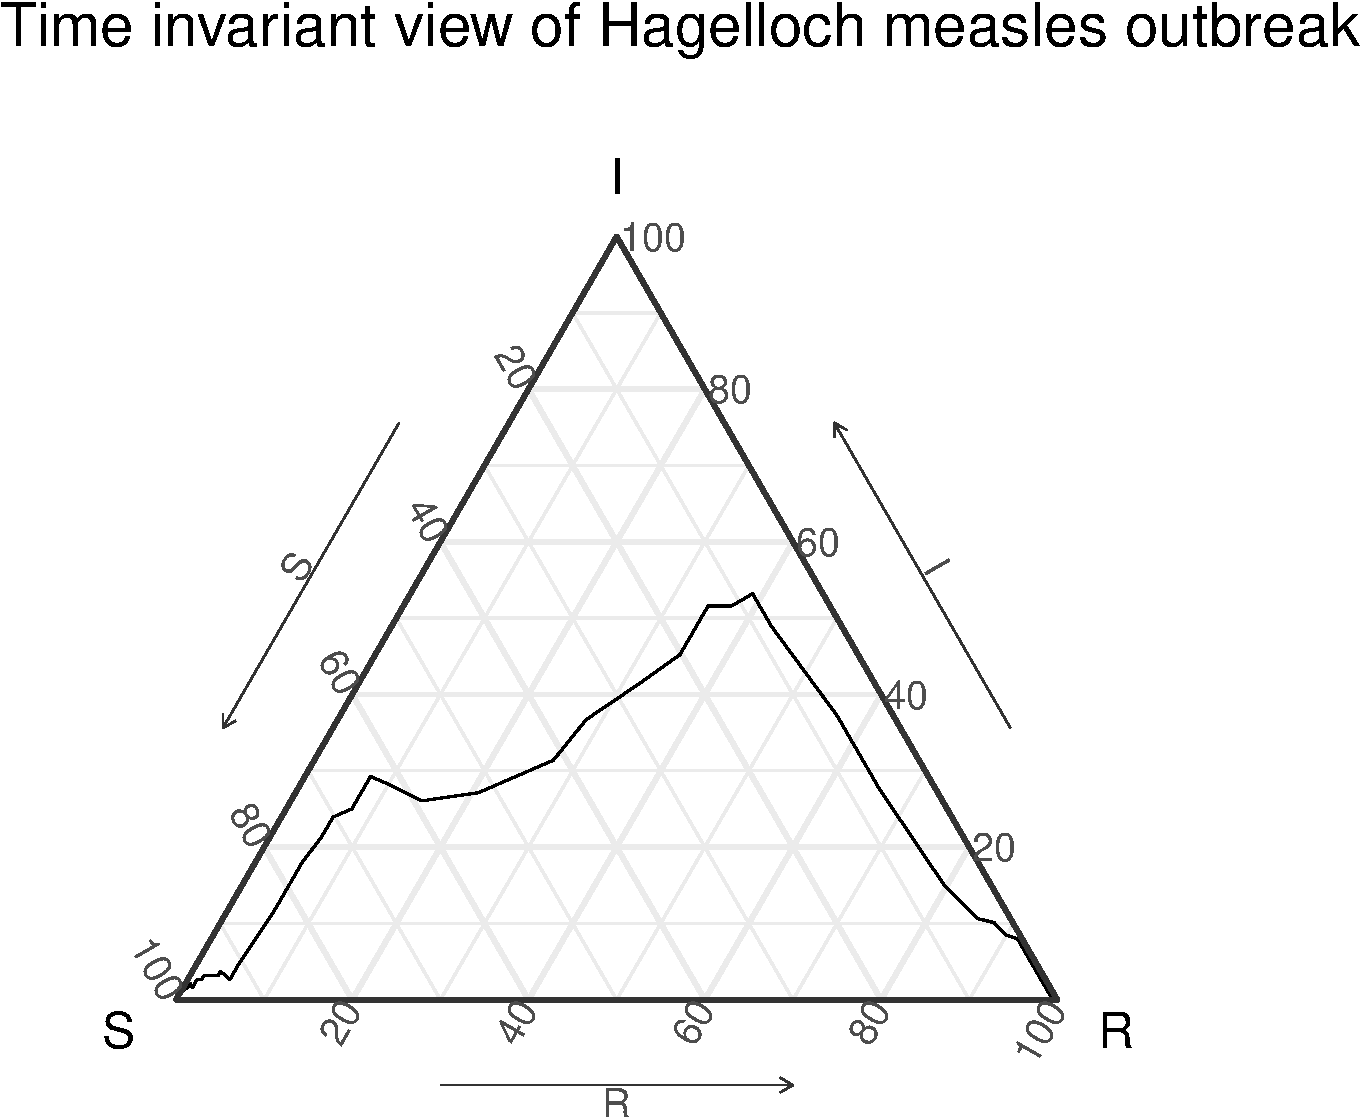
\includegraphics{Figs/unnamed-chunk-9-1} 

}

\caption{\label{fig:hag-tern-raw}Time invariant view of the Hagelloch epidemic where we view the individuals in Susceptible, Infectious, or Recovered states.  We see there are two peaks of infection (the vertical axis).}\label{fig:unnamed-chunk-9}
\end{figure}
\end{CodeChunk}

Moreover, we can look at the outbreaks of the disease by group within
\code{agent_to_aggregate()} or \code{geom_aggregate()}. This allows us
to examine differences among the different groups of individuals. For
example, we show the time invariant outbreak by class level in Figure
\ref{fig:tern-class-data}. Immediately, we see that time invariant
infection curve is different for the pre-school class compared to the
1st class. In the 1st class, we see about 95\% of the class become
infected and less than 10\% of them having recovered, which may be
indicative of a super-spreading event. This suspicion is further
confirmed in that 26 of the 30 1st class students have been reportedly
infected by the same individual.

\begin{CodeChunk}
\begin{CodeInput}
R> hagelloch_raw %>%
+   ggplot(aes(y = tI, z = tR, color = CL)) +
+   geom_aggregate(size = 2) + coord_tern() +
+   labs(x = "S", y = "I", z = "R",
+        color = "Class") +
+   scale_color_brewer(palette = "Dark2") +
+   facet_wrap(~CL)
\end{CodeInput}
\begin{figure}[H]

{\centering 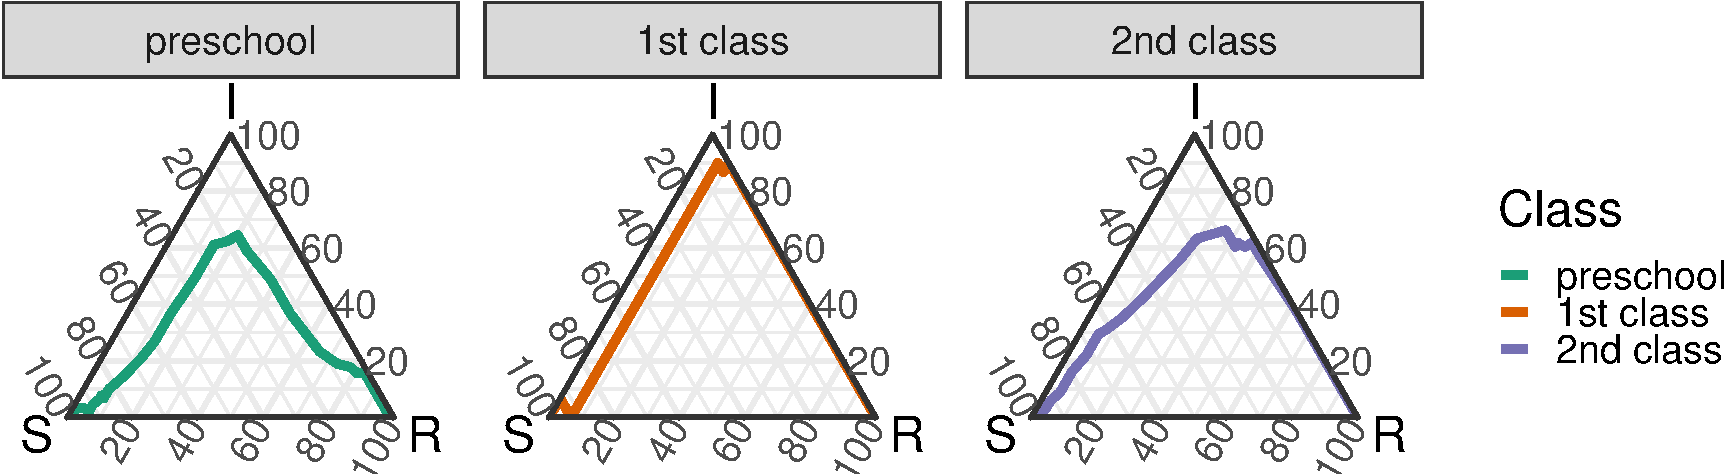
\includegraphics{Figs/unnamed-chunk-10-1} 

}

\caption{\label{fig:tern-class-data}Time invariant outbreak curves for the three class groups.  The pre-school class has a distinct peak of infection whereas the peak infection point for the other two classes are less well defined.}\label{fig:unnamed-chunk-10}
\end{figure}
\end{CodeChunk}

Along with multiple epidemic states, the function
\code{agents_to_aggregate()} can also be extended to populations with
vital dynamics (e.g.~birth and death) and examples of this are shown in
the package vignette. In summary, \code{agents_to_aggregate()} is a
multi-purpose workhorse that may be leveraged to convert individual
level records into aggregate information that may be more useful for
some forms of epidemic modeling such as compartment modeling.

\hypertarget{modeling-and-simulation}{%
\subsection{Modeling and Simulation}\label{modeling-and-simulation}}

\footnote{\textcolor{orange}{section headings to align with our pipeline}}

Up to this point, we have used \pkg{EpiCompare} in the context of
observed data. We also want to compare statistical models, and
\pkg{EpiCompare} aids in that process via a simple yet flexible
individual-level
simulator\sout{, conversion tools for popular epidemic model packages, and model assessments.}
We demonstrate an example here.

We first try to model the Hagelloch data with a stochastic SIR model,
which we refer to as the `simple SIR.' In our full vignette
\textcolor{orange}{(available online),} we show how to fit this simple
SIR model via maximum likelihood and simulate from the model with those
best fit parameters. Our function \code{simulate_agents()} generates
individual level data according to discrete time multinomial draws,
which depend on the number of individuals in each state at the previous
time step and a matrix of transition probabilities. For example, the
below code generates 100 simulations of an outbreak of a disease with
one initial infector in a population of \(n= 188\) individuals.

\begin{CodeChunk}
\begin{CodeInput}
R> trans_mat <- matrix(c("X0 * (1 - X1 * par1 / N)", "X0 * X1  * par1 / N", "0",
+                   "0", "X1 * (1 - par2)", "par2 * X1",
+                   "0", "0", "X2"), byrow = TRUE, nrow = 3)
\end{CodeInput}
\end{CodeChunk}

\begin{CodeChunk}
\begin{CodeInput}
R> set.seed(2020)
R> 
R> best_params <- c("beta" = .36, "gamma" = .13)
R> ## This is the SIR representation
R> 
R> rownames(trans_mat) <- c("S", "I", "R")
R> init_vals <- c(187, 1, 0)
R> par_vals <- c(par1 = best_params[1], par2 = best_params[2])
R> max_T <- 55
R> n_sims <- 100
R> 
R> agents <- simulate_agents(trans_mat,
+                        init_vals,
+                        par_vals,
+                        max_T,
+                        n_sims,
+                        verbose = FALSE)
\end{CodeInput}
\end{CodeChunk}

\begin{CodeChunk}
\begin{CodeInput}
R> agg_model <- agents %>% group_by(sim) %>%
+   agents_to_aggregate(states = c(I, R)) %>%
+   mutate(Type = "Simple SIR")
\end{CodeInput}
\end{CodeChunk}

The result of our simulation is the object \code{agents} which is a
18800 \(\times\) 5 data frame, which details the time of entry into the
\(S\), \(I\), and \(R\) states for a given simulation. Before we examine
the results of this simple SIR model, we will also examine another, more
sophisticated SIR model, this time from the package \pkg{EpiModel}
\citep{Jenness2018}. Briefly, this model first fits a contact network to
the set of individuals, where the class of the child is a covariate. The
model then simulates a SIR-epidemic on that network.

\begin{CodeChunk}
\begin{CodeInput}
R> library(EpiModel)
R> ## WARNING:  Will take a minute or two
R> 
R> set.seed(42)
R> nw <- network.initialize(n = 188, directed = FALSE)
R> nw <- set.vertex.attribute(nw, "group", rep(0:2, each = 90, 30, 68))
R> formation <- ~edges + nodematch("group") + concurrent
R> target.stats <- c(200, 300, 200)
R> coef.diss <- dissolution_coefs(dissolution = ~offset(edges),  duration = 5)
R> est1 <- netest(nw, formation, target.stats, coef.diss, edapprox = TRUE)
R> 
R> param <- param.net(inf.prob = 0.1, act.rate = 5, rec.rate = 0.1)
R> status.vector <- c(rep(0, 90), rep(0, 30), rep(0, 67), 1)
R> status.vector <- ifelse(status.vector == 1, "i", "s")
R> init <- init.net(status.vector = status.vector)
R> control <- control.net(type = "SIR", nsteps = 55,
+                        nsims = 100, epi.by = "group")
R> epimodel_sir <- netsim(est1, param, init, control)
\end{CodeInput}
\end{CodeChunk}

The output of this model is \code{epimodel_sir}, an object of class
\code{netsim}, which contains a plethora of modeling information.

\hypertarget{post-processing-and-comparison}{%
\subsection{Post-processing and
comparison}\label{post-processing-and-comparison}}

The next step is to compare the Simple SIR model to the EpiModel SIR
model. We provide the function \code{fortify_aggregate()}, which can
take objects from specialized classes of modeling output
\textcolor{orange}{(like those made by \code{netsim()})} and transform
it into a tidy-style data frame.

\begin{CodeChunk}
\begin{CodeInput}
R> fortified_net <- fortify_aggregate(epimodel_sir, 
+                                    states = c("s.num", "i.num", "r.num")) %>%
+   mutate(Type = "EpiModel SIR",
+          sim = as.numeric(gsub("sim", "", sim)))
\end{CodeInput}
\end{CodeChunk}

We can then analyze the results of the two models side by side as
time-invariant epidemic curves. The results are shown in Figure
\ref{fig:hag-simple-sir}, where a 90\% prediction band is estimated from
the delta ball method for each of the two models. For the Simple SIR
model, we see that the data generally covers the data fairly well but
clearly misses the second peak of infection. We also see that the
prediction band is very large, covering up a large area of the ternary
plot. On the other hand, for the EpiModel network model, we see that the
prediction band covers the data quite well and takes up less area.

\begin{CodeChunk}
\begin{CodeInput}
R> both_models <- bind_rows(agg_model, fortified_net)
R> 
R> 
R> g <- ggplot() + geom_prediction_band(data = both_models %>% filter(t != 0),
+          aes(x = X0, y = X1, z = X2,
+               sim_group = sim, fill = Type),
+          alpha = .5,
+          conf_level = .90) 
\end{CodeInput}
\end{CodeChunk}

\begin{CodeChunk}
\begin{CodeInput}
R> g +   geom_path(data = both_models %>% filter(t !=0),
+             aes(x = X0, y = X1, z = X2, group = paste(Type, sim)),
+             alpha = .3, col = "gray40") + 
+     coord_tern() + theme_sir(base_size = 24) +
+   geom_point(data = hagelloch_sir,
+              aes(x = S, y = I, z =R), col = "black") +
+   labs(title = "Simple SIR model",
+        subtitle = "90% Prediction band and original data",
+        x = "S", y = "I", z = "R") +
+   scale_fill_manual(values = c("#006677", "#AA6600")) + 
+   facet_wrap(~Type) +
+   theme(legend.position = "bottom")
\end{CodeInput}
\begin{figure}[H]

{\centering 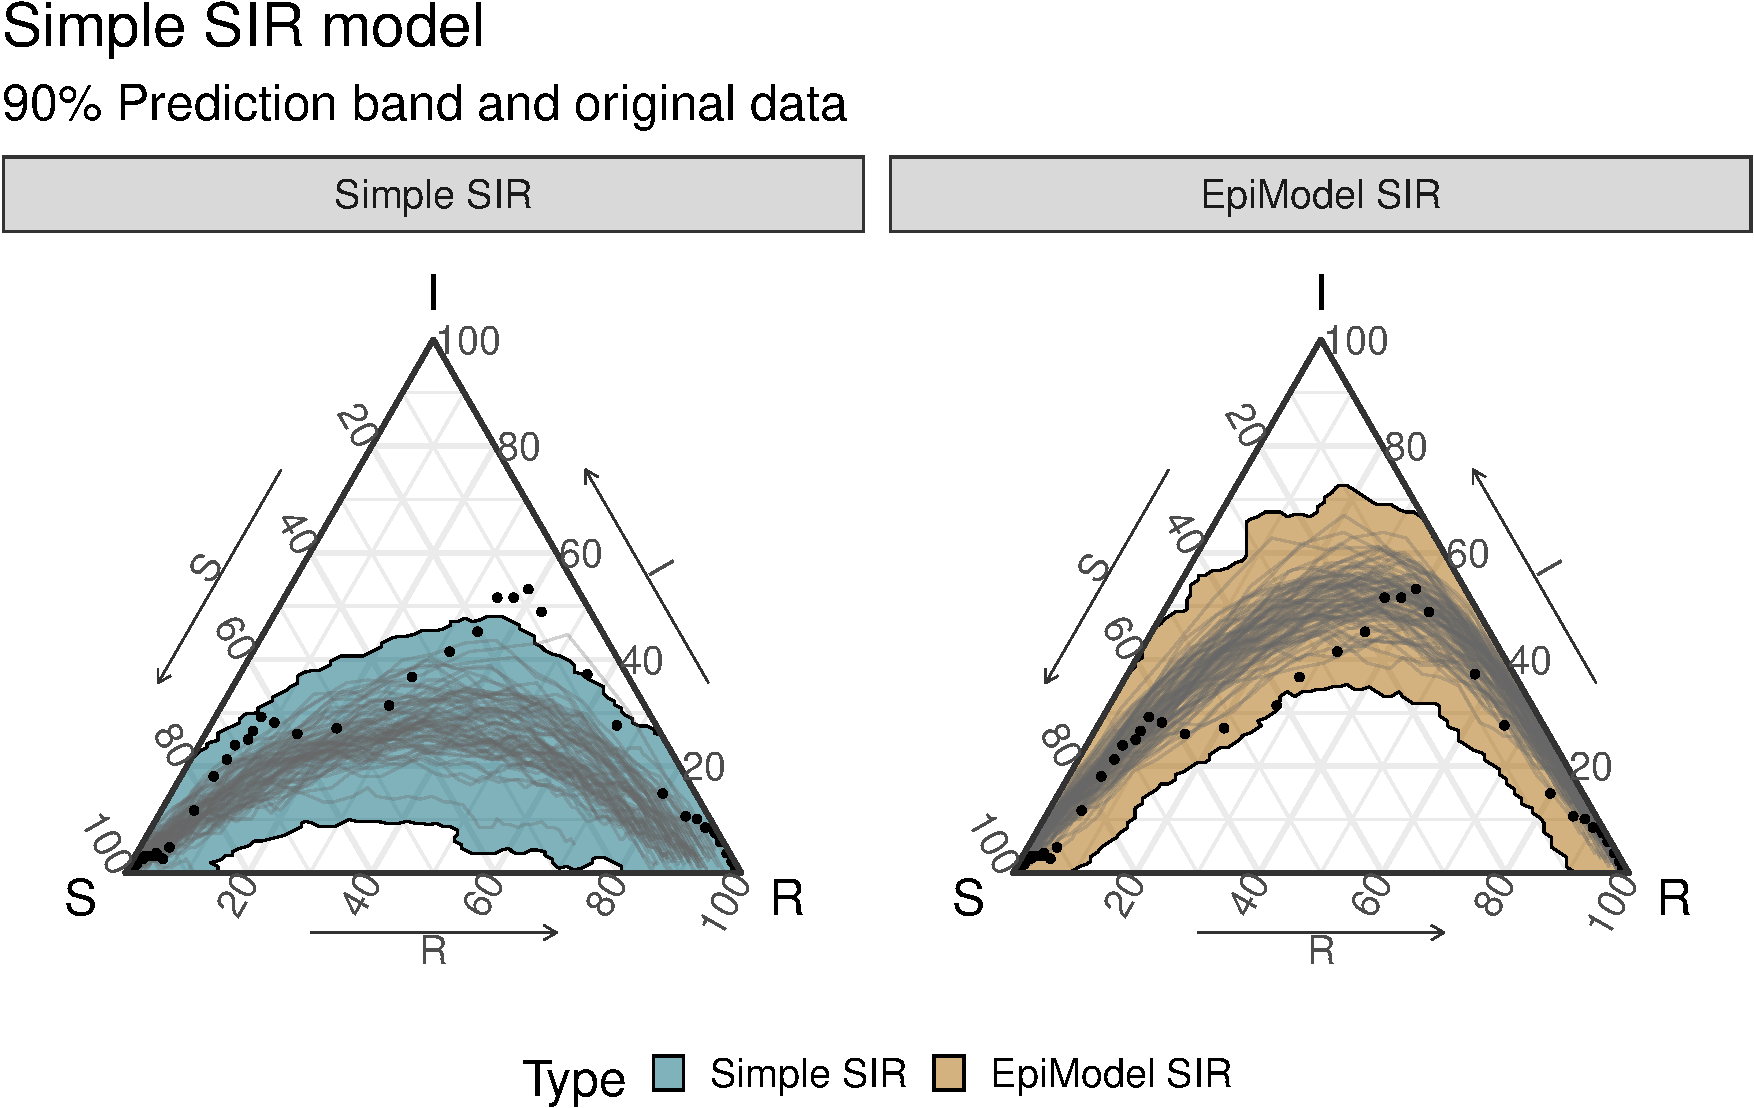
\includegraphics{Figs/unnamed-chunk-17-1} 

}

\caption{\label{fig:hag-simple-sir}  Original Hagelloch SIR data (black) along with 90\% prediction band and actual simulation paths from the Simple SIR and the EpiModel SIR models.}\label{fig:unnamed-chunk-17}
\end{figure}
\end{CodeChunk}

However, both models are not a good fit to the filamental path as
opposed to the individual points in \((S, I, R)\)-space. This can be
captured with the set of simulations both models predict (gray lines),
which all generally have a single defined peak of infection whereas the
data certainly looks like it has two distinct peaks, likely caused by
our assumed super-spreader event. This observation is backed up by the
below analysis that demonstrates that the estimated pseudo-density of
the observed epidemic (relative to the simulations from either model) is
much less likely then \textbf{any} of the simulations (reported in Table
\ref{tab:hags-extreme})\footnote{\textcolor{orange}{Ben, do we want to add another sentence or two explaining the two columns in the table?  The second one I think makes sense to me but not the first.}}
In conclusion, \pkg{EpiCompare} makes it clear that, at a glance, 1) the
EpiModel network model is a better fit than the Simple SIR model, and 2)
the fit is only good at the
\sout{geometric filamental level as opposed to the epidemic trajectory filamental level.}
\textcolor{orange}{individual point level as opposed to the geometric filamental level.}

\begin{CodeChunk}
\begin{CodeInput}
R> #-- after cleaning up and combining --
R> all_together_df <- rbind(simple_sir,
+                          hagelloch_sir2)
\end{CodeInput}
\end{CodeChunk}

\begin{CodeChunk}
\begin{table}[!h]

\caption{\label{tab:cif-all-together-df}Top and bottom 2 rows of \tt{all\_together\_df}\textnormal{, combining both simulated epidemics and the true epidemic.}}
\centering
\begin{tabular}[t]{lrrrrr}
\toprule
Type & sim & t & S & I & R\\
\midrule
Simple SIR & 1 & 0 & 188 & 0 & 0\\
Simple SIR & 1 & 1 & 187 & 1 & 0\\
true observation & 0 & 54 & 1 & 0 & 187\\
true observation & 0 & 55 & 1 & 0 & 187\\
\bottomrule
\end{tabular}
\end{table}

\end{CodeChunk}

\begin{CodeChunk}
\begin{CodeInput}
R> compression_df <- all_together_df %>% group_by(Type, sim) %>% 
+   filament_compression(data_columns = c("S","I","R"), 
+                        number_points = 20)
\end{CodeInput}
\end{CodeChunk}

\begin{CodeChunk}
\begin{CodeInput}
R> tdmat <- compression_df %>% 
+   dist_matrix_innersq_direction(
+     position = c(1:length(compression_df))[
+       names(compression_df) %in% c("S","I", "R")],
+     tdm_out = T)
R> 
R> simple_sir_true_obs_info <- tdmat %>% 
+   compare_new_to_rest_via_distance(
+     new_name_id = data.frame(Type = "true observation", sim = 0),
+     distance_func = distance_psuedo_density_function, 
+     sigma = "20%") 
\end{CodeInput}
\end{CodeChunk}

\begin{CodeChunk}
\begin{table}[!h]

\caption{\label{tab:hags-extreme}The extremeness of the true simulations based on comparing pseudo-density estimates between true vs simulated curves}
\centering
\begin{tabular}[t]{l>{\raggedleft\arraybackslash}p{6cm}>{\raggedleft\arraybackslash}p{6cm}}
\toprule
Type & simulations-based estimated pseudo-density & proportion of simulations with lower estimated pseudo-density\\
\midrule
Simple SIR & 0.0036733 & 0.00\\
EpiModel SIR & 0.0149686 & 0.02\\
\bottomrule
\end{tabular}
\end{table}

\end{CodeChunk}

Overall, \pkg{EpiCompare} aids in the data analysis pipeline for both
novice and expert practitioners and coders alike. These tools encourage
model and simulation exploration of many of the existing and
well-supported packages that already exist, and side-by-side comparison
thereof. Finally, we hope that practicioners will consider using
time-invariant analysis when trying to assess and compare epidemics and
epidemic models.

\hypertarget{a.-appendix}{%
\section*{A. Appendix}\label{a.-appendix}}
\addcontentsline{toc}{section}{A. Appendix}

\hypertarget{a.1-proof-of-theorem}{%
\subsection*{\texorpdfstring{A.1 Proof of Theorem
\ref{thm:sir-scale}}{A.1 Proof of Theorem }}\label{a.1-proof-of-theorem}}
\addcontentsline{toc}{subsection}{A.1 Proof of Theorem
\ref{thm:sir-scale}}

\begin{proof}\label{proof:thm}
\cite{Harko2014} provide an analytical solution for the Kermack and McKendrick equations (Eq. \eqref{eq:sir-ode}) by reparameterizing the ODEs so that $\mathcal{S}(u) = S(t)$, $\mathcal{I}(u) = S(t)$, and $\mathcal{R}(u) = R(t)$ for $0< u_T < 1$ with
\begin{align}\label{eq:harko-odes}
\mathcal{S}(u) &= S(0)u\\
\mathcal{I}(u) &= N - R(0) + NR_0^{-1}\log u - S(0)u \nonumber\\
\mathcal{R}(u) &= R(0) - NR_0^{-1} \log u, \nonumber
\end{align}
and $u$ and t are related by the following integral,
\begin{align*}
    t &= \int_{u}^1 \frac{N}{\beta \tau (N - R(0) + R_{0}^{-1} \log \tau - S(0)\tau)}d\tau \\
    &= \int_{u}^1 \frac{1}{\beta f(S(0), R(0), N, R_0, \tau)} d \tau\\
    &= \int_{u}^1 \frac{1}{\beta f(\tau)} d\tau,
\end{align*}
where we have made the denominator of the integral a function of $N$, the initial values, $R_0$, and $\tau$, which we further condense to $f(\tau)$ for brevity.
Then for a given $t$ we want to find $s$ such that $(S_1(t), I_1(t), R_1(t)) = (S_2(s), I_2(s), R_2(s))$.  Or equivalently, for a fixed $u$ want to find $v$ such that  $\mathcal{S}_1(u) = \mathcal{S}_2(v)$ and then the corresponding $t$ and $s$ are given by
\begin{align*}
    t & = \int_{u}^1 \frac{1}{\beta_1 f(\tau)} d\tau \\
    s & = \int_{v}^1 \frac{1}{\beta_2 f(\tau)} d\tau.
\end{align*}
Note that since the equations in Eq. \eqref{eq:harko-odes} are functions of the initial values and $R_0$, then $u = v$. We then can find a relation for $s$,
    \begin{align*}
    s & = \int_{u}^1 \frac{1}{\beta_2 f(\tau)} d\tau  \\
    & = \int_{u}^1 \frac{1}{a\beta_1 f(\tau)} d\tau \\ 
    &= \frac{1}{a}\int_{u}^1 \frac{1}{\beta_1 f(\tau)} d\tau \\
    &= \frac{1}{a}t.
\end{align*}
\end{proof}

\bibliography{EpiCompare.bib}


\end{document}
